\documentclass[a4paper,german]{article}
%Partially taken from
%https://github.com/gillescastel/university-setup/blob/master/preamble.tex
%but edited for own purposes

% Some basic packages
\usepackage[ngerman]{babel}
\usepackage[T1]{fontenc}
\usepackage[mathletters]{ucs}
\usepackage[utf8x]{inputenc}
\usepackage{textcomp}
\usepackage{url}
\usepackage{graphicx}
\usepackage{float}
\usepackage{booktabs}
\usepackage[shortlabels]{enumitem}
\usepackage{hyperref}



\makeatletter
\newcommand\setItemnumber[1]{\setcounter{enum\romannumeral\@enumdepth}{\numexpr#1-1\relax}}
\makeatother

% for wrapping text around figures
\usepackage{wrapfig}


\pdfminorversion=7

% Don't indent paragraphs, leave some space between them
\usepackage{parskip}

% Hide page number when page is empty
\usepackage{emptypage}
\usepackage{subcaption}
\usepackage{multicol}
% Other font I sometimes use.
\usepackage{xcolor}
\usepackage{comment}
% \usepackage{cmbright}

% Math stuff
\usepackage{amsmath, amsfonts, mathtools, amsthm, amssymb}
% Fancy script capitals
\usepackage{mathrsfs}
\usepackage{cancel}
% Bold math
\usepackage{bm}
% Some shortcuts
\newcommand\N{\ensuremath{\mathbb{N}}}
\newcommand\R{\ensuremath{\mathbb{R}}}
\newcommand\Z{\ensuremath{\mathbb{Z}}}
\renewcommand\O{\ensuremath{\emptyset}}
\newcommand\Q{\ensuremath{\mathbb{Q}}}
\newcommand\C{\ensuremath{\mathbb{C}}}

% Easily typeset systems of equations (French package)
\usepackage{systeme}

% Put x \to \infty below \lim
\let\svlim\lim\def\lim{\svlim\limits}

%Make implies and impliedby shorter
\let\implies\Rightarrow
\let\impliedby\Leftarrow
\let\iff\Leftrightarrow
\let\epsilon\varepsilon

% Add \contra symbol to denote contradiction
\usepackage{stmaryrd} % for \lightning
\newcommand\contra{\scalebox{1.5}{$\lightning$}}

% \let\phi\varphi

% Command for short corrections
% Usage: 1+1=\correct{3}{2}

\definecolor{correct}{HTML}{009900}
\newcommand\correct[2]{\ensuremath{\:}{\color{red}{#1}}\ensuremath{\to }{\color{correct}{#2}}\ensuremath{\:}}
\newcommand\green[1]{{\color{correct}{#1}}}

% horizontal rule
\newcommand\hr{
    \noindent\rule[0.5ex]{\linewidth}{0.5pt}
}

% hide parts
\newcommand\hide[1]{}

% si unitx
\usepackage{siunitx}
\sisetup{locale = FR}

%Theorem-environments
\usepackage{mdframed}
\mdfsetup{skipabove=\topskip,skipbelow=\topskip}

\newtheoremstyle{own}%〈name〉
{3pt}%〈Space above〉1
{3pt}%〈Space below〉1
{}%〈Body font〉
{}%〈Indent amount〉2
{\bfseries}%〈Theorem head font〉
{.}%〈Punctuation after theorem head〉
{.5em}%〈Space after theorem head〉3
{}%〈Theorem head spec(can be left empty, meaning ‘normal’)〉

\theoremstyle{own}

\global\mdfdefinestyle{thm}{linecolor=red,linewidth=2pt,leftmargin=0cm,rightmargin=0cm, backgroundcolor=red!8, rightline=false, topline=false, bottomline=false}

\global\mdfdefinestyle{lemma}{linecolor=orange,linewidth=2pt,leftmargin=0cm,rightmargin=0cm, backgroundcolor=orange!10, rightline=false, topline=false, bottomline=false}

\global\mdfdefinestyle{definition}{linecolor=blue,linewidth=2pt,leftmargin=0cm,rightmargin=0cm, backgroundcolor=blue!7, rightline=false, topline=false, bottomline=false}

\global\mdfdefinestyle{example}{linecolor=green!70!black,linewidth=2pt,leftmargin=0cm,rightmargin=0cm, rightline=false, topline=false, bottomline=false}

\global\mdfdefinestyle{remark}{linecolor=yellow!80!orange,linewidth=2pt,leftmargin=0cm,rightmargin=0cm, rightline=false, topline=false, bottomline=false}


\global\mdfdefinestyle{notation}{linecolor=violet,linewidth=2pt,leftmargin=0cm,rightmargin=0cm, backgroundcolor=violet!7, rightline=false, topline=false, bottomline=false}

\global\mdfdefinestyle{theoremdef}{linecolor=red,linewidth=2pt,leftmargin=0cm,rightmargin=0cm, backgroundcolor=blue!7, rightline=false, topline=false, bottomline=false}

\newtheorem{protothm}{Theorem}[section]
\newenvironment{theorem}{\begin{mdframed}[style=thm] \begin{protothm}}{\end{protothm}\end{mdframed}}

\newtheorem*{protothm*}{Theorem}
\newenvironment{theorem*}{\begin{mdframed}[style=thm] \begin{protothm*}}{\end{protothm*}\end{mdframed}}

\newtheorem{protoprop}[protothm]{Proposition}
\newenvironment{proposition}{\begin{mdframed}[style=thm] \begin{protoprop}}{\end{protoprop}\end{mdframed}}



\newtheorem{protocor}[protothm]{Corollary}
\newenvironment{corollary}{\begin{mdframed}[style=thm] \begin{protocor}}{\end{protocor}\end{mdframed}}

\newtheorem{protolemma}[protothm]{Lemma}
\newenvironment{lemma}{\begin{mdframed}[style=lemma] \begin{protolemma}}{\end{protolemma}\end{mdframed}}

\newtheorem*{protlemma*}{Lemma}
\newenvironment{lemma*}{\begin{mdframed}[style=lemma] \begin{protolemma*}}{\end{protolemma*}\end{mdframed}}

\newtheorem{protodefinition}[protothm]{Definition}
\newenvironment{definition}{\begin{mdframed}[style=definition] \begin{protodefinition}}{\end{protodefinition}\end{mdframed}}


\newtheorem{prototheoremdef}[protothm]{Theorem and Definition}
\newenvironment{theoremdef}{\begin{mdframed}[style=theoremdef] \begin{prototheoremdef}}{\end{prototheoremdef}\end{mdframed}}


\newtheorem*{protodefinition*}{Definition}
\newenvironment{definition*}{\begin{mdframed}[style=definition] \begin{protodefinition*}}{\end{protodefinition*}\end{mdframed}}

\newtheorem*{protonotation}{Notation}
\newenvironment{notation}{\begin{mdframed}[style=notation] \begin{protonotation}}{\end{protonotation}\end{mdframed}}

\newtheorem*{protoexample}{Example}
\newenvironment{example}{\begin{mdframed}[style=example] \begin{protoexample}}{\end{protoexample}\end{mdframed}}

\newtheorem*{protoremark}{Remark}
\newenvironment{remark}{\begin{mdframed}[style=remark] \begin{protoremark}}{\end{protoremark}\end{mdframed}}

% Recaps
\usepackage[skins]{tcolorbox}

\newtcolorbox{recap}{before skip = 0.5cm, after skip = 0.5cm, enhanced, sharp corners = all, colback = white, colframe = gray, toprule=0pt, bottomrule=0pt, leftrule=0pt,rightrule=0pt, overlay = {
        \draw[gray, line width = 2pt] (frame.north west) -- ++(0.5cm, 0pt);
        \draw[gray, line width=2pt] (frame.south east) -- ++(-0.5cm, 0pt);
        \draw[gray, line width=2pt] (frame.north west) -- ++ (0pt, -0.5cm);
        \draw[gray, line width=2pt] (frame.south east) -- ++(0pt, 0.5cm);
}}



% Environments
\makeatother
% For box around Definition, Theorem, \ldots
\theoremstyle{definition}
\newtheorem*{problem}{Problem}

\newtheorem*{previouslyseen}{As previously seen}
\newtheorem*{warning}{\color{red} Warning}
\newtheorem*{info}{Information}
\newtheorem*{claim}{Claim}
\newtheorem*{moral}{Moral}
\newtheorem*{tday}{Plan for today}
\newtheorem*{aim}{Ziel}
\newtheorem*{summary}{So far}
\newtheorem*{fact}{Fact}
\newtheorem*{exercise}{Exercise}
\newtheorem*{nxt}{Next}
\newtheorem*{note}{Note}
\newtheorem*{question}{Question}
\newtheorem*{answer}{Answer}
\newtheorem*{observe}{Observe}
\newtheorem*{property}{Property}
\newtheorem*{intuition}{Intuition}
\newtheorem*{goal}{Goal}
\newtheorem*{recall}{Recall}
\newtheorem*{idea}{Idea}

% End example and intermezzo environments with a small diamond (just like proof
% environments end with a small square)
\usepackage{etoolbox}
\AtEndEnvironment{example}{\null\hfill$\diamond$}%
% \AtEndEnvironment{opmerking}{\null\hfill$\diamond$}%

% Fix some spacing
% http://tex.stackexchange.com/questions/22119/how-can-i-change-the-spacing-before-theorems-with-amsthm
\makeatletter
\def\thm@space@setup{%
  \thm@preskip=\parskip \thm@postskip=0pt
}


% Exercise 
% Usage:
% \oefening{5}
% \suboefening{1}
% \suboefening{2}
% \suboefening{3}
% gives
% Oefening 5
%   Oefening 5.1
%   Oefening 5.2
%   Oefening 5.3
\newcommand{\oefening}[1]{%
    \def\@oefening{#1}%
    \subsection*{Oefening #1}
}

\newcommand{\suboefening}[1]{%
    \subsubsection*{Oefening \@oefening.#1}
}


% \lecture starts a new lecture (les in dutch)
%
% Usage:
% \lecture{1}{di 12 feb 2019 16:00}{Inleiding}
%
% This adds a section heading with the number / title of the lecture and a
% margin paragraph with the date.

% I use \dateparts here to hide the year (2019). This way, I can easily parse
% the date of each lecture unambiguously while still having a human-friendly
% short format printed to the pdf.

\usepackage{xifthen}
\def\testdateparts#1{\dateparts#1\relax}
\def\dateparts#1 #2 #3 #4 #5\relax{
    \marginpar{\small\textsf{\mbox{#1 #2 #3 #5}}}
}

\def\@lecture{}%
\newcommand{\lecture}[3]{
    \ifthenelse{\isempty{#3}}{%
        \def\@lecture{Lecture #1}%
    }{%
        \def\@lecture{Lecture #1: #3}%
    }%
    \subsection*{\@lecture}
    \marginpar{\small\textsf{\mbox{#2}}}
}



% These are the fancy headers
\usepackage{fancyhdr}
\pagestyle{fancy}

% LE: left even
% RO: right odd
% CE, CO: center even, center odd
% My name for when I print my lecture notes to use for an open book exam.
% \fancyhead[LE,RO]{Gilles Castel}

\fancyhead[RO,LE]{\@lecture} % Right odd,  Left even
\fancyhead[RE,LO]{}          % Right even, Left odd

\fancyfoot[RO,LE]{\thepage}  % Right odd,  Left even
\fancyfoot[RE,LO]{}          % Right even, Left odd
\fancyfoot[C]{\leftmark}     % Center

\makeatother




% Todonotes and inline notes in fancy boxes
\usepackage{todonotes}
\usepackage{tcolorbox}

% Make boxes breakable
\tcbuselibrary{breakable}

% Verbetering is correction in Dutch
% Usage: 
% \begin{verbetering}
%     Lorem ipsum dolor sit amet, consetetur sadipscing elitr, sed diam nonumy eirmod
%     tempor invidunt ut labore et dolore magna aliquyam erat, sed diam voluptua. At
%     vero eos et accusam et justo duo dolores et ea rebum. Stet clita kasd gubergren,
%     no sea takimata sanctus est Lorem ipsum dolor sit amet.
% \end{verbetering}
\newenvironment{verbetering}{\begin{tcolorbox}[
    arc=0mm,
    colback=white,
    colframe=green!60!black,
    title=Opmerking,
    fonttitle=\sffamily,
    breakable
]}{\end{tcolorbox}}

% Noot is note in Dutch. Same as 'verbetering' but color of box is different
\newenvironment{noot}[1]{\begin{tcolorbox}[
    arc=0mm,
    colback=white,
    colframe=white!60!black,
    title=#1,
    fonttitle=\sffamily,
    breakable
]}{\end{tcolorbox}}




% Figure support as explained in my blog post.
\usepackage{import}
\usepackage{xifthen}
\usepackage{pdfpages}
\usepackage{transparent}
\newcommand{\incfig}[1]{%
    \def\svgwidth{\columnwidth}
    \import{./figures/}{#1.pdf_tex}
}

% Fix some stuff
% %http://tex.stackexchange.com/questions/76273/multiple-pdfs-with-page-group-included-in-a-single-page-warning
\pdfsuppresswarningpagegroup=1


% My name
\author{Maximilian Keßler}




\DeclarePairedDelimiter\abs{\lvert}{\rvert}
\DeclareMathOperator{\id}{id}
\DeclareMathOperator{\coker}{coker}
\DeclareMathOperator{\dz}{dz}
\DeclareMathOperator{\diam}{diam}
\DeclareMathOperator{\ex}{ex}
\DeclareMathOperator{\dt}{dt}
\DeclareMathOperator{\dist}{dist}
\DeclareMathOperator{\Ext}{Ext}
\DeclareMathOperator{\Tor}{Tor}
\DeclareMathOperator{\supp}{supp}
\DeclareMathOperator{\im}{im}
\DeclareMathOperator{\Lip}{Lip}
\DeclareMathOperator{\Mspec}{MaxSpec}
\DeclareMathOperator{\Proj}{Proj}
\DeclareMathOperator{\QCoh}{QCoh}
\renewcommand\Im\im
\DeclareMathOperator{\Mor}{Mor}
\DeclareMathOperator{\Hom}{Hom}
\DeclareMathOperator{\Gal}{Gal}
\DeclareMathOperator{\MaxSpec}{MaxSpec}
\DeclareMathOperator{\Aut}{Aut}
\DeclareMathOperator{\dy}{dy}
\DeclareMathOperator{\Fun}{Fun}
\DeclareMathOperator{\Presh}{Pre-Sh}
\DeclareMathOperator{\Sh}{Sh}
\DeclareMathOperator{\dif}{diff}
\DeclareMathOperator{\opp}{opp}
\DeclareMathOperator{\Ob}{Ob}

\newcommand*\circled[1]{\tikz[baseline=(char.base)]{
            \node[shape=circle,draw,inner sep=2pt] (char) {#1};}}

            \usepackage[ngerman,ruled,vlined]{algorithm2e}

\newcommand{\vocab}[1]{\textbf{\color{blue} #1}}

\usepackage{tikz-cd}
\newcommand{\cat}[1]{ \mathscr{#1} }


\title{Algorithmische Mathematik II}
\author{{\normalsize Dozent} \\ {\sc Professor Dr. Patrik Ferrari}}
\usepackage{bbm}

\begin{document}
    \maketitle
    \vspace{3em}
    \centering \small Version \\
    \today\; \currenttime
    \vspace{10em}
    \abstract{Bei folgenden Vorlesungsnotizen handelt es sich um (inoffizielle) Mitschriften zur Vorlesung 'Algorithmische Mathematik II', die im Sommersemester 2021 an der Universität Bonn gehalten wird. Ich garantiere weder für Korrektheit noch Vollständigkeit dieser Notizen, und bin dankbar für jegliche Art von Korrektur, sowohl inhaltlich, als auch Tippfehler. \\
Bemerkungen, die nicht zum eigentlichen Vorlesungsinhalt gehören, wurden mit einem * gekennzeichnet. Sie werden nach eigenem Ermessen hinzugefügt, um weitere Details oder evtl. mündliche Anmerkungen beizufügen. \\
Manche Umgebungen sind mit einem $^{\dagger}$ versehen. Das ist dann der Fall, wenn ihr Inhalt so, oder zumindest in sehr ähnlicher Form, in der Vorlesung vorkam (unter Umständen auch mündlich), ich aber die Umgebung der Aussage geändert habe. Insbesondere also, wenn ich aus Aussagen, die einfach erwähnt werden, ein \textbf{Lemma$^{\dagger}$} mache, um sie hervorzuheben. \\
Weitere Informationen finden sich bei \href{https://github.com/kesslermaximilian/LectureNotesBonn}{GitHub} oder auf der \href{https://wt.iam.uni-bonn.de/ferrari/teaching/lectures-homepages/almaiiss19-1}{Vorlesungshomepage}

    \newpage
    \tableofcontents
    \newpage
    \listoflecture
    \addcontentsline{toc}{section}{Übersicht der Vorlesungen}
    \newpage
    % start lectures
    \lecture[Motivationsfragen. Brown'sche Bewegung. Ereignisse, Wahrscheinlichkeiten, Modell von Zufallsexperimenten.]{Mo 12 Apr 2021 10:16}{Grundbegriffe}

\begin{itemize}
    \item Es gibt einen Helpdesk, auch explizit einen nur für Studentinnen.
    \item Die Vorlesung wird aufgenommen, und zwar ohne Videos der Teilnehmenden sowie des Dozenten. Die Aufzeichnungen werden anschließend in Sciebo hochgeladen.
    \item Es gibt ein Diskussionsforum für Fragen (auf eCampus).
    \item Ab heute Abend, 18 Uhr (Mo 12 Apr 2021 18:00), kann man sich auf eCampus für die Übungsgruppen registrieren und dies endet am Dienstag Abend um 24 Uhr (Di 12 Apr 2021 24:00) - es wird versucht, die Studenten gleichmäßig zu verteilen.
    \item Falls ihr in der Warteliste landet und gewünscht ist, in der Gruppe abzugeben, schreibt eine Mail mit den gewünschten Abgabepartnern, dann kann eine gemeinse Einteilung erfolgen.
    \item Es gibt auch das Modul \verb?AlmaIIb?. Registriert euch noch nicht, dies ist für den 2. Teil der Vorlesung notwendig. 
    \item Die Abgabe der Übungsblätter erfolgt einheitlich jeden Freitag um 12 Uhr.
    \item Gruppenabgaben sind erlaubt, bis zu einer Größe von maximal 4 StudentInnen.
    \item Das 1. Blatt ist freiwillig und gibt Bonuspunkte.
    \item Für die Klausurzulassung werden 50\% der Punkte benötigt. Von den Programmieraufgaben müssen mindestens 4 von 6 zufriedenstellend bearbeitet werden.
    \item Programmieraufgaben gibt es ab dem 2. Übungsblatt auf jedem 2. Blatt. Die Bearbeitungszeit beträgt dann 2 Wochen.
\end{itemize}


\section*{Einleitung}
In der Vorlesung wird folgendes betrachtet werden:
\begin{description}
    \item[Teil 1: Diskrete Stochastik]
        \begin{itemize}
            \item Zufallsvariablen
            \item Bedingte Wahrscheinlichkeiten
            \item Unabhängigkeit von Variablen
            \item Monte-Carlo Methoden
        \end{itemize}
    \item[Teil 2: Numerische Analysis]
        \begin{itemize}
            \item Iterative Verfahren
            \item Interpolation von Daten (durch Polynome, trigonometrische Funktionen, \ldots)
            \item Numerische Verfahren für die Integration
        \end{itemize}
\end{description}


\section{Diskrete Stochastik}
\subsection{Einleitung}
\begin{goal}
    Beschreibung von Systemen, die einen Anteil an \vocab{Zufall} haben, d.h. nicht 100\% deterministisch sind.
\end{goal}
\begin{example}
    \begin{itemize}
        \item Spiele: Kartenspiele, Glücksspiele, \ldots
        \item Statistik: Umfragen, Versicherungen
        \item Komplexe Systeme: Wettermodelle, Finanzmärkte
    \end{itemize}
\end{example}

\underline{Was sind Quellen von Zufall?}
\begin{itemize}
    \item Zu komplexe Systeme: Zufälliges Aussehen des Gesamteffekts
    \item Fehlende Informationen (z.B. bei einem Kartenspiel)
    \item Chaotische Systeme (beispielsweise das Wetter)
    \item Intrinsisch unvorhersagbare Systeme (z.B. radioaktiver Zerfall)
\end{itemize}
\begin{question}
    \begin{enumerate}[(1)]
        \item Wie modelliert man ein System mit Zufall?
        \item Wie simuliert man ein System mit Zufall? (anwendungstechnischer)
        \item Welche Voraussagen kann man machen?
    \end{enumerate}
\end{question}


\begin{example}
    Die \vocab{Brown'sche Bewegung}. Das System ist implizit ein Pollen mit vielen Wassermolekülen ($\sim 10^{23})$, die sich im Prinzip deterministisch bewegen. \\
    $\implies$ Wir erhalten ein Gleichungssystem mit $(N+1)\cdot 6$ (3 Positionen, 3 Geschwindigkeit) Variablen. Dieses ist de facto unlösbar. \\

    Was wollen wir hier eigentlich untersuchen? -> Die Bewegung des Pollens, jedoch nicht die der einzelnen Wassermoleküle. \\
    In einer \vocab{Modellierung} ersetzt man die Stöße, die durch die Wassermoleküle entstehen, durch \vocab{zufällige Stöße}. 
\end{example}

\underline{Diskretes Modell:} Die Zeit bewegt sich in $n\in \left \{0,1,2,\ldots\right\} $. Sei
\[
    Z(n) := (\text{Position des Pollens zur Zeit $n$}) \in  \Z^3
.\] 
OBdA setzen wir $Z(0) = 0$. \\
\underline{Dynamik}: $Z(n+1) = Z(n) + \xi_n$, wobei wir $\xi_n$ aus dem Ergebnis eines Würfelwurfs bestimmen werden:
 \[
\xi_n = \begin{cases}
    (1,0,0) & \text{wenn Würfel}=1 \\
    (-1,0,0) & \text{wenn Würfel}=2 \\
    (0,1,0) & \text{wenn Würfel}=3 \\
    (0,-1,0) & \text{wenn Würfel}=4 \\
    (0,0,1) & \text{wenn Würfel}=5 \\
    (0,0,-1) & \text{wenn Würfel}=6
\end{cases}
.\] 

\begin{question}
    Welche Fragen können wir mit solch einem System nun beantworten? Was pasiert, wenn $n\gg 1$?
\end{question}
\begin{enumerate}[\protect\circled{\alph*}]
    \item Typischerweise erhalten wir $\abs{Z(n)} =  O(\sqrt{n}) $ 
    \item Wenn wir die Frequenz von $[Z(n)]_i$ betrachten, (d.h. bei welcher Koordinate in Richtung $i$ befinden wir uns nach  $n$ Würfen) sehen wir typischerweise: 
        \begin{figure}[h]
            \centering
\begin{tikzpicture}[
    declare function={binom(\k,\n,\p)=\n!/(\k!*(\n-\k)!)*\p^\k*(1-\p)^(\n-\k);}
]
\begin{axis}[
    samples at={-15,...,15},
    yticklabel style={
        /pgf/number format/fixed,
        /pgf/number format/fixed zerofill,
        /pgf/number format/precision=2
    },
    ybar=0pt, bar width=1
]
\addplot [fill=orange, fill opacity=0.5] {binom(x+30,60,0.5)}; \addlegendentry{$[Z(n)]_i$}
    \addplot[draw=red,thick,smooth] {1/(sqrt(30*pi)) *exp(-1/30*x^2)}; \addlegendentry{\text{Gaussglocke}}
\end{axis}
\end{tikzpicture}
\caption{Binomialverteilung und Gaussglocke}
\end{figure}
Für $n\gg 1$ sieht diese Verteilung dann ungefähr wie die Gaussglocke aus. \\
\end{enumerate}
\underline{Skalierung:} Wir setzen nun
\[
    B(t) = \lim_{n \to \infty} \frac{Z(\left\lfloor nt \right\rfloor )}{\sqrt{n} }
.\] 
und dies ist dann die Brownsche Bewegung.

Nun möchten wir Vorhersagen treffen können:
\begin{question}
        Ist $Z(n)$ in einer gegebenen Menge  $A$?
\end{question}
Das kann man (im Allgemeinen) nicht einfach mit 'Ja' oder 'Nein' beantworten. Stattdessen müssen wir fragen:
\begin{question}
Wenn man $Z(n)$ beobachtet, wie häufig wird  $Z(n)$ in  $A$ sein?
\end{question}
Diese Frage lässt sich mit einer Zahl $\in [0,1]$ beantworten.

\subsection{Ereignisse und Wahrscheinlichkeiten}
Wir benötigen 3 Grundelemente:
\begin{enumerate}[(1)]
    \item Die Menge $\Omega$ von möglichen \vocab{Ergebnissen}. die Elemente von $\Omega$ heißen auch  \vocab{Elementarereignisse}.
    \item Die Menge $\mathcal{F}$ der \vocab{Ereignisse}. Ein Ereignis  $E$ ist eine Eigenschaft, die mit einer Teilmenge $G\subset \Omega$ assoziiert ist: $ω\in G \iff $ Eigenschaft $E$ ist erfüllt.
    \item Eine \vocab{Wahrscheinlichkeitsverteilung (auch W-maß)}:
        \[
            \mathbb{P}: \mathcal{F} \to  [0,1]
        .\] 
\end{enumerate}
\begin{remark*}
    Wir werden noch sehen, dass gewisse Dinge für unsere Begriffe erfüllt sein müssen, dazu aber später mehr.
\end{remark*}

\begin{example}
    Eine Urne hat 12 nummerierte Kugeln (von 1 bis 12).
    \begin{enumerate}[(1)]
        \item Das \vocab{Zufallsexperiment} besteht daraus, dass wir eine Kugel aus der Urne ziehen und die Zahl notieren, die wir sehen. D.h.
            \[
            \Omega = \left \{1,\ldots,12\right\} 
            .\] 
            Ein Elementarereignis ist nun z.B. gegeben durch $ω = \left \{5\right\}  \equiv 5$ (wir vereinfachen die Notation).
        \item Mögliche Ereignisse sind z.B:
            \begin{equation}
                \begin{split}
                    A &= \text{'Die Zahl ist gerade'} \\
                    B&= \text{'Die Zahl ist }\leq 5 \text{'}\\
                    C &= \text{'Die Zahl ist 8'}
                \end{split}
            \end{equation}
            Die assoziierten Mengen sind dann
            \begin{equation}
                \begin{split}
                    A &= \left \{2,4,6,8,10,12\right\}  \\
                     B &= \left \{1,2,3,4,5\right\} \\
                      C & = \left \{8\right\} 
                \end{split}
            \end{equation}
        \item Für die Wahrscheinlichkeiten nehmen wir an, dass jede Kugel die gleiche Chance hat, gezogen zu werden, d.h.
            \[
                \forall G\in \mathcal{F}: \mathbb{P}(G) = \frac{\abs{G}}{\abs{\Omega} }
            .\] 
            Wir erhalten nun die Wahrscheinlichkeiten
            \[
                \mathbb{P}(A) = \frac{6}{12}=\frac{1}{2} \qquad \mathbb{P}(B) = \frac{5}{12} \qquad \mathbb{P}(C) = \frac{1}{12}
            .\] 
    \end{enumerate}
\end{example}

\begin{notation}
    $A\equiv \left \{ω\in \Omega \mid  ω\in A\right\} \equiv  \left \{ω\in A\right\} \equiv \left \{A \text{ tritt ein}\right\} $
\end{notation}







    \lecture[$σ$-Algebren, Messräume. Wahrscheinlichkeitsverteilungen, Wahrscheinlichkeitsräume. Einschluss-Ausschluss-Prinzip. Endliche (diskrete) Wahrscheinlichkeitsräume.]{Mi 14 Apr 2021 10:17}{}
Wir kennen nun die Grundbegriffe $\Omega, \mathcal{F}, \mathbb{P}$ zur Beschreibung von Zufallsexperimenten, die wir uns nun genauer ansehen wollen:
\begin{question}
    Welche Struktur muss $\mathcal{F}$ besitzen.
\end{question}
Sein $A,B\in \mathcal{F}$, dann können wir das Ereignis $A \cap B$ betrachten, d.h. beide der Eigeschaften treten ein. Genauso sollte
 \[
A^{c} := \Omega \setminus A 
.\] 
, das \vocab{Komplement von $A$}, bzw. das \vocab{Gegenereignis} von $A$ ebenfalls in  $\mathcal{F}$  sein. Aus den beiden vorherigen Eigenschaften folgt bereits, dass
\[
    A \cup B= (A^{c} \cap B^{c})^{c}
.\] 
ebenfalls in $\mathcal{F}$ sein wird. \\
Eine Menge $\mathcal{F}$ mit solchen Eigenschaften heißt \vocab{Algebra}.
\begin{dnotation}
Seien nun $A,B$ und $(A_i)_{i\in I}$  Ereignisse, wobei $I$ endlich oder abzählbar sei. Dann notieren wir die folgenden Ereignisse:
\begin{enumerate}[label=\protect\circled{\alph*}]
    \item \emphasize{$A \cup B$} : $ω\in A \cup B \iff  ω\in A \lor ω\in B$, d.h. $A\cup B$ tritt ein, genau dann, wenn  $A$ eintritt oder  $B$ eintritt.
        \item  \emphasize{$\bigcup_{i \in  I} A_i$}: $ω\in \bigcup_{i \in  I} A_i$, wenn es ein $i\in I$ gibt, sodass $\omega \in A_i$
    \item  \emphasize{$A \cap B$}: $\omega\in A \cap B \iff  $ A \underline{und} B treten ein.
        \item \emphasize{$\bigcap_{i \in I} A_i$}: $\omega\in \bigcap_{i \in I}A_i \iff \forall i \in I \colon$ $A_i$ tritt ein.
            \item \emphasize{$A = \emptyset$} ist das Ereignis, das  \underline{nie} eintritt. \\
                \emphasize{$A = \Omega$} ist das Ereignis, dass \underline{immer} eintritt.
\end{enumerate}
\end{dnotation}

\begin{definition}[$\sigma$-Algebra]\label{def:sigma-algebra}
    Eine  \vocab{$\sigma$-Algebra} ist eine nicht leere Menge $\mathcal{F}$ von Teilmengen von $\Omega$ mit den Eigenschaften:
    \begin{enumerate}[label=\protect\circled{\alph*}]
        \item $\Omega \in \mathcal{F}$
        \item $\forall A\in \mathcal{F} \colon A^{c}\in \mathcal{F}$.
        \item Falls $(A_i)_{i \in I}\in \mathcal{F}$, dann auch $\bigcup_{i=1} ^{\infty}A_i \in \mathcal{F}$
    \end{enumerate}
    Wir nennen $(\Omega,\mathcal{F})$ dann einen \vocab{Messraum}. 
\end{definition}

\begin{lemma}\label{lm:weitere-eigenschaften-einer-sigma-algebra}
    Sei $\mathcal{F}$ eine $\sigma$-Algebra, dann ist:
    \begin{enumerate}[label=\protect\circled{\alph*}]
        \item $\emptyset\in \mathcal{F}$
        \item $A,B \in \mathcal{F} \implies A \cup B \in \mathcal{F}$ und $A\cap B \in \mathcal{F}$.
        \item $(A_i)_{i \in I}\in \mathcal{F} \implies \bigcap_{i=1}^{\infty}A_i \in \mathcal{F}$.
    \end{enumerate}
\end{lemma}
\begin{proof}
    \begin{enumerate}[label=\protect\circled{\alph*}]
        \item $\emptyset = \Omega^{c} \in \mathcal{F}$ nach Eigenschaften \circled{a} und \circled{b} aus der Definition.
        \item $A \cup B = A \cup B \cup \emptyset \cup \emptyset \ldots \in \mathcal{F}$ nach Eigenschaften  \circled{b} und \circled{c}. $A \cap B = (A^{c}\cup B ^{c})^{c} \in \mathcal{F}$
        \item $\bigcap_{i=1}^{\infty}A_i = \left( \bigcup_{i=1}^{\infty}A_i^{c} \right) ^{c}\in \mathcal{F}$ nach \circled{b} und \circled{c}.
    \end{enumerate}
\end{proof}

Wir haben nun $(\Omega, \mathcal{F})$ näher untersucht, es fehlt nun noch $\mathbb{P}$. 
\begin{question}
    Welche Eigenschaften soll $\mathbb{P}$ (das Wahrscheinlichkeitsmaß bzw. die Wahrscheinlichkeitsverteilung) besitzen?
\end{question}
Seien $A,B \in \mathcal{F}$ mit $A\cap B = \emptyset$, d.h. $A$ und $B$ können nicht gleichzeitig eintreten. Dann fordern wir
\[
    \mathbb{P}(A \cap B) = \mathbb{P}(A) + \mathbb{P}(B) \quad \text{(endliche Additivität)}
.\] 
Dazu wollen wir, dass $\Omega \in \mathcal{F}$ immer eintritt, d.h. $\mathbb{P}(\Omega) = 1 \equiv  100\%$ (Normierung).

\begin{definition}[Wahrscheinlichkeitsverteilung]\label{def:wahrscheinlichkeitsverteilung}
Sei $(\Omega, \mathcal{F})$ ein Messraum. Eine Abbildung $\mathbb{P} : \mathcal{F} \to  \R_+$ ist eine \vocab{Wahrscheinlichkeitsverteilung} auf $(\Omega, \mathcal{F})$, falls
    \begin{enumerate}[(1)]
        \item $\mathbb{P}(\Omega) = 1$
        \item Sind $(A_i)_{i \in I}\in \mathcal{F}$ paarweise disjunkt, so ist:
            \[
                \mathbb{P}\left( \bigcup_{i=1}^{\infty}A_i \right) = \sum_{i=1}^{\infty} \mathbb{P}(A_i) \quad (\sigma\text{-Additivität})
            .\] 
    \end{enumerate}
\end{definition}
\begin{remark*}
    Die Definition macht implizit Gebrauch davon, dass die linke Seite überhaupt definiert ist. Dies folgt jedochdaraus, dass $\mathcal{F}$ eine $\sigma$-Algebra ist.
\end{remark*}

\begin{definition}[Wahrscheinlichkeitsraum]\label{def:wahrscheinlichkeitsraum}
    Ein \vocab{Wahrscheinlichkeitsraum $(\Omega, \mathcal{F},\mathbb{P})$} besteht aus einer Menge $\Omega$, einer  $\sigma$-Algebra $F\subset \mathbb{P}\mathcal{(\Omega)}$ und einem Wahrschenilichkeitsmass $\mathbb{P}$ auf $(\Omega, \mathcal{F})$ 
\end{definition}


\begin{lemma}\label{lm:weitere-eigenschaften-eines-wahrscheinlichkeitsraums}
    Sei $(\Omega, \mathcal{F}, \mathbb{P})$ ein Wahrscheinlichkeitsraum. Dann ist
\begin{enumerate}[label=\protect\circled{\alph*}]
    \item $\mathbb{P}(\emptyset)=0$ 
    \item $\forall A,B\in \mathcal{F}$ mit $A\cap B = \emptyset$ ist
        \[
            \mathbb{P}(A\cup B ) = \mathbb{P}(A) + \mathbb{P}(B)
        .\] 
    \item      $\forall A,B\in \mathcal{F}$ mit $A\subset B$ ist 
        \begin{equation*}
            \begin{split}
                \mathbb{P}(B) &= \mathbb{P}(A) + \mathbb{P}(B \setminus A)  \\
                \mathbb{P}(A^{c}) &= 1 - \mathbb{P}(A) \\
                \mathbb{P}(A) &\leq  \mathbb{P}(B) \leq  1
            \end{split}
        \end{equation*}
    \item $\forall A,B \in \mathcal{F}$ ist
        \begin{equation*}
            \begin{split}
                \mathbb{P}(A \cup B) &= \mathbb{P}(A) + \mathbb{P}(B) - \mathbb{P}(A\cap B) \\
                                     &\leq  \mathbb{P}(A) + \mathbb{P}(B)
            \end{split}
        \end{equation*}
    \item Wenn $A_n \nearrow A$ ,d.h. $A_1\subset A_2\subset \ldots$ mit $\bigcup_{i =1}^{\infty} A_i = A$ (monotone Konvergenz von Mengen), oder $A_n \searrow A$ (d.h.  $A_1\supset A_2 \supset \ldots$ mit $\bigcap_{i=1}^{\infty} A_i = A $ ), so ist
        \[
            \lim_{n \to \infty} \mathbb{P}(A_n) = \mathbb{P}\left( \lim_{n \to \infty} A_n \right)  = \mathbb{P}(A)
        .\] 
\end{enumerate}
\end{lemma}
\begin{proof}
    \begin{enumerate}[label=\protect\circled{\alph*}]
        \item Wir wissen:
            \[
                1= \mathbb{P}(\Omega) = \mathbb{P}\left( \Omega \cup \emptyset \cup \emptyset \cup \emptyset \ldots  \right)  = \mathbb{P}(\Omega) + \mathbb{P}(\emptyset) + \mathbb{P}(\emptyset) + \ldots
            .\] 
            subtrahieren von $\mathbb{P}(\Omega) =1$ liefert dann $\mathbb{P}(\emptyset) = 0$.
        \item Sei $A \cap B = \emptyset$, dann ist:
            \begin{equation*}
                \begin{split}
                    \mathbb{P}(A\cup B ) &= \mathbb{P}(A \cup B \cup \emptyset \cup \emptyset \cup \ldots) \\
                                         &\stackrel{σ-\text{Additivität}}{=} \mathbb{P}(A) + \mathbb{P}(B) + \mathbb{P}(\emptyset) + \mathbb{P}(\emptyset) + \ldots \\
                                         &= \mathbb{P}(A) + \mathbb{P}(B)
                \end{split}
            \end{equation*}
        \item Sei $A\subset B$. Dann ist $B = A \cup (B \setminus A)$ eine disjunkte Vereinigung, also erhalten wir
            \[
                \mathbb{P}(B) = \mathbb{P}(A) + \underbrace{\mathbb{P}(B \setminus A)}_{\geq 0} \geq  \mathbb{P}(A)
            .\] 
            Mit $B = \Omega$ ergibt sich  $1 = \mathbb{P}(A) + \mathbb{P}(A^{c})$
        \item Es ist
            \begin{equation}
                \begin{split}
                    \mathbb{P}(A \cup B) &= \mathbb{P}(A) + \mathbb{P}((A \cup B) \setminus A)  \\
                                         &= \mathbb{P}(A) + \mathbb{P}(B \setminus (A \cap B)) \\
                                         &= \mathbb{P}(A) + \mathbb{P}(B) - \underbrace{\mathbb{P}(A \cap B)}_{\geq 0} \\
                                         &\geq \mathbb{P}(A) + \mathbb{P}(B)
                \end{split}
            \end{equation}
        \item Übung
    \end{enumerate}
\end{proof}
\begin{corollary}[Einschluss-Ausschluss-Prinzip]\label{cor:einschluss-ausschluss-prinzip}
    Seien $A_1,\ldots,A_n \in \mathcal{F}$. Dann gilt
    \[
        \mathbb{P}(A_1 \cup \ldots \cup A_n) = \sum_{k=1}^{n} (-1)^{k-1} \sum_{1\leq i_1<i_2<\ldots<i_k \leq n} \mathbb{P}(A_{i_1} \cap A_{i_2} \cap \ldots \cap A_{i_k})
    .\] 
\end{corollary}
\begin{proof}
    Per Induktion, der Induktionsanfang lautet  $\mathbb{P}(A_1) = \mathbb{P}(A_1)$ und ist offensichtlich wahr. \\
    Die Aussage gelte nun für ein $n\in \N$, dann erhalten wir
    \begin{equation}
        \begin{split}
            \mathbb{P}\left( \bigcup_{i=1}^{n+1} A_i \right)  &= \mathbb{P}\left( \left(\bigcup_{i=1}^{n}A_i \right) \cup A_{n+1}\right)  \\
                                                              &= \mathbb{P}\left(\bigcup_{i=1}^{n} A_i\right) + \mathbb{P}(A_{n+1}) - \mathbb{P}\left( \left( \bigcup_{i=1}^n A_i \right) \cap A_{n+1} \right)  \\
                                                              &= \mathbb{P}\left( \bigcup_{i=1}^{n} A_i \right)  + \mathbb{P}(A_{n+1}) - \mathbb{P}\left( \bigcup_{i=1}^n \underbrace{(A_i \cap _{A_{n+1}})}_{=: \tilde{A}_i} \right)  \\
                                                              &= \sum_{k=1}^{n} (-1)^{k-1} \sum_{1\leq i<\ldots<i_k \leq n} \mathbb{P}(A_{i_1} \cap \ldots \cap A_{i_k}) + \mathbb{P}(A_{n+1}) \\
                                                              &\qquad -\sum_{k=1}^n (-1)^{k-1} \sum_{1\leq i_1 < \ldots < i_k \leq n} \mathbb{P}(\underbrace{\tilde{A}_{i_1} \cap \ldots \cap \tilde{A}_{i_k}}_{A_{i_1} \cap \ldots \cap A_{i_k} \cap A_{n+1}})
        \end{split}
    \end{equation}
    Andererseits ist aber auch:
    \begin{alignat*}{5}
           &\quad&  &\sum_{k=1} ^{n+1} (-1)^{k-1} \sum_{1\leq i_1<\ldots<i_k \leq  n+1} \mathbb{P}(A_{i_1} \cap \ldots \cap A_{i_k}) &\quad & \\
           &= & &\sum\limits_{k=1}^{n}(-1)^{k-1} \sum\limits_{1\leq i_1< \ldots < i_k \leq  \color{red} n} \mathbb{P}(A_{i_1} \cap \ldots \cap A_{i_k}) & \quad &\Big\}\text{\parbox{2cm}{Terme mit $i_k\leq n$}} \\
           &+& &\underbrace{\sum_{k=2}^{n+2} (-1)^{k-1} \sum_{1\leq i_1<\ldots<i_{k-1}\leq n} \mathbb{P}(A_i \cap \ldots \cap A_{i_{k-1}} \cap A_{n+1})}_{\stackrel{l := k-1}{=} -\sum\limits_{l=1}^n (-1)^{l-1}\sum\limits_{1\leq i_1<...<i_l\leq n} \mathbb{P}(A_{i_1} \cap \ldots \cap A_{i_l} \cap A_{n+1})}& \quad &\Bigg\}\text{\parbox{2cm}{\small Terme mit $i_k = n+1$ und  $k\geq 2$}}\\
           &+& & \mathbb{P}(A_{n+1}) \qquad& \quad  &\Big\}\text{\parbox{2cm}{\small Terme mit $i_k = n+1$ und  $k=1$}}
    \end{alignat*}
    und damit sehen wir, dass die beiden Ausdrücke übereinstimmen, also ist der Induktionsschritt erbracht.
\end{proof}


\subsection{Diskrete Verteilungen}
\begin{itemize}
    \item Sei nun $\Omega$ endlich oder abzählbar.
    \item Falls wir $\mathcal{F}$ nicht explizit angeben, dann wird $\mathcal{F} = \mathcal{P}(\Omega)$ gewählt, d.h.
        \[
            \operatorname{Card} (\mathcal{P}(\Omega)) \equiv \abs{\mathcal{P}(\Omega)} = 2 ^{ \abs{\Omega}} 
        .\] 
\end{itemize}
\begin{example}[Münzwurf]
    Es sei $\Omega = \left \{K,Z\right\}$, wobei $K$ für Kopf stehe und $Z$ für Zahl. Dann ist
    \[
    \mathcal{F} = \left \{\left \{K\right\} ,\left \{Z\right\} ,\left \{Z,K\right\} ,\emptyset\right\} 
    .\] 
    Sei $p\in [0,1]$ die Wahrscheinlichkeit, dass man Kopf erhält. Da $\mathbb{P}$ für alle Element aus $\mathcal{F}$ definiert sein muss, erhalten wir
    \[
        \mathbb{P}(\emptyset) = 0 \qquad \mathbb{P}(K) = p, \qquad \mathbb{P}(Z) = \mathbb{P}(K^{c}) = 1-p \qquad \mathbb{P}(\left \{Z,K\right\} ) = \mathbb{P}(\Omega) = 1
    .\] 
\end{example}
\begin{question}[Charakterisierung von diskreter Wahrscheinlichkeit]
Was müssen wir fordern, sodass $\mathbb{P}$ auf $\mathcal{P}(\Omega)$ gibt?.
\end{question}
\begin{example}
    $\Omega = \left \{1,2,\ldots,10\right\}$ würde genügen, da dann $\abs{\mathcal{P}(\Omega)}= 2^{\abs{\Omega} }=2^{10} = 1024 $
    endlich (diskret) ist.
\end{example}

    \lecture[Diskrete Verteilungen. Gleichverteilung. Fixpunkte von Permutationen. Empirische Verteilung.]{Mo 19 Apr 2021 10:23}{Gleichverteilung, empirische Verteilung}
Wir stellen fest, dass es im letzten Beispiel auch genügt hätte, $\mathbb{P}(\left \{k\right\} )$ für $k=1,\ldots,10$ anzugeben. Daraus ergibt sich:
\begin{theorem}\label{thm:wahrscheinlichkeitsverteilungen-auf-abzaehlbaren-raeumen}
    \begin{enumerate}[label=\protect\circled{\alph*}]
        Sei $\Omega$ abzählbar.
        \item Sei $p(\omega)\in [0,1], \omega\in \Omega$, sodass
            \[
                \sum_{\omega\in \Omega}p(\omega) = 1
            .\] 
            Dann ist $\mathbb{P}$ definiert durch:
                \begin{equation*}
                \mathbb{P}: \left| \begin{array}{c c l} 
                    \mathcal{P}(\Omega) & \longrightarrow & [0,1] \\
                    A & \longmapsto &  \sum_{\omega\in A}p(\omega)
                \end{array} \right.
            \end{equation*}
            eine Wahrscheinlichkeitsverteilung auf $(\Omega,\mathcal{P}(\emptyset))$. 
        \item Jede Wahrscheinlichkeitsverteilung $\mathbb{P}$ auf $(\Omega,\mathcal{P}(\Omega))$ hat obige Form, wobei $p(\omega) = \mathbb{P}(\left \{\omega\right\} )$.
    \end{enumerate}
\end{theorem}

\begin{remark}
    $p:\emptyset\to [0,1]$ heißt Massenfunktion der Wahrscheinlichkeitsverteilung $\mathbb{P}$. \\
    \warning Der Satz gilt nicht für $\Omega$ überabzählbar.
\end{remark}


\begin{remark}
    Sei $A$ abzählbar und  $p(\omega) \geq 0$ für $\omega\in A$. Dann definiert
    \[
        \sum_{\omega\in A} p(\omega) := \sum_{k\geq 1} p(\omega_k)
    .\] 
    mit einer beliebigen Abzählung $\omega_1,\omega_2, \ldots, \omega_k$ von $A$ eine wohldefinierte Summe der  $p(\omega)$. Es ist wichtig, dass hier $p(\omega) \geq 0$, sonst wäre obiges nicht wohldefiniert.
\end{remark}

\begin{lemma}\label{lm:approximation-von-massen-durch-endliche-teilmengen}
        Sei  $A$ abzählbar.
    \begin{enumerate}[label=\protect\circled{\alph*}]
        \item Sei $p(\omega) \in [0,1]$ für alle $\omega$. Dann ist
            \[
                \sum_{\omega\in A} p(\omega) \in [0,\infty]
            .\] 
            wohldefiniert. Setzen wir
            \[
                \mathbb{P}(A) := \sum_{\omega\in A} p(w)
            .\] 
            so gilt
            \[
                P(A) = \sup_{\substack{F\subset A \\ \abs{F} <\infty}} P(F)
            .\] 
            und $P(A) \leq  P(B)$ für $A\subset B$.
        \item Ist $A = \bigsqcup_{k=1}^{\infty} A_k$ eine disjunkte Vereinigung, so ist
            \[
                P(A) = \sum_{k=1}^{\infty}P(A_k)
            .\] 
    \end{enumerate}
\end{lemma}
\begin{proof}
    \begin{enumerate}[label=\protect\circled{\alph*}]
        \item Sei $\omega_1,\omega_2,\ldots$ eine beliebige Abzählung von $A$. Dann ist die Funktion
             \[
                 n \longmapsto \sum_{k=1}^n p(\omega_k)
            .\] 
            monoton wachsend. Also ist
            \[
                \sum_{k=1}^{\infty} p(\omega_k) := \lim_{n\to \infty}\sum_{k=1}^{n} p(\omega_k) = \sup_{n\in \N} \sum_{k=1}^n p(\omega_k) \in [0,\infty]
            .\]
            wohldefiniert. \\
            Wir wollen nun noch zeigen, dass 
            \[
                P(A) := \sum_{k=1}^{\infty} p(\omega_k) \stackrel{!}{=} \sup_{\substack{F\subset A \\ \abs{F} <\infty} }P(F)
            .\] 
            Die Ungleichung '$\leq $' folgt sofort, da mit $F_n := \left \{\omega_1, \ldots, \omega_k\right\} $ folgt
            \[
                \sum_{k=1}^n p(\omega_k) = \sum_{\omega\in F_n} p(\omega) = P(F_n) \leq  \sup_{\substack{F\subset A \\ \abs{F} <\infty} } P(F)
            .\] 
            Also ergibt sich im Limes genau wie gewünscht
            \[
                P(A) = \lim_{n\to \infty} \sum_{k=1}^n p(\omega_k) \leq  \lim_{n\to \infty} \sup_{\substack{F\subset A\\ \abs{F} <\infty} }P(F) = \sup_{\substack{F\subset A\\ \abs{F} <\infty} }P(F)
            .\] 
            Für '$\geq $' stellen wir fest, dass es für jedes $F\subset A$ endlich ein $n\in \N$ gibt, sodass $F\subset \left \{\omega_1,\ldots,\omega_n\right\} $ und somit gilt
            \[
                P(F) = \sum_{\omega\in F} P(\omega) \leq  \sum_{k=1}^n p(\omega_k) \leq  \sum_{k=1}^{\infty} p(\omega_k) = P(A)
            .\] 
            Damit ist das Supremum der $P(F)$ für $F\subset A, \abs{F} <\infty$ durch $P(A)$ beschränkt. \\
            Für die letzte Behauptung sehen wir mit $A\subset B$ leicht, dass
            \[
                P(A) = \sup_{\substack{F\subset A \\ \abs{F} <\infty} } P(F) \leq  \sup_{\substack{ F\subset B \\ \abs{F} <\infty}} = P(B)
            .\] 
        \item ($\sigma$-Additivität) Wir unterscheiden zwischen zwei Fälle:
            \begin{enumerate}[1)]
                \item Falls $\abs{A} <\infty$, so ist $A = \bigsqcup_{k=1}^n A_k$ für ein $n$, und somit gilt
                    \begin{equation}
                        \begin{split}
                            P(A) &= \sum_{l=1}^{\abs{A} }p(\omega_l) = \sum_{l=1}^{\abs{A} } \sum_{k=1}^{n} p(\omega_l) \mathbb{1}_{A_k}(\omega_l)  \\
                                          &= \sum_{k=1}^{n} \sum_{l=1}^{\abs{A} } p(\omega_l) \mathbb{1}_{A_k}(\omega_l) = \sum_{k=1}^n P(A_k)
                        \end{split}
                    \end{equation}
                \item Sei nun $\abs{A} =\infty$. Wir zeigen zunächst '$\leq $'. Für ein endliches $F\subset A$ ist
                    \[
                        F = \bigcup_{k=1}^{\infty} (F \cap A_k)
                    .\] 
                    eine disjunkte Vereinigung mit endlich vielen Termen, also ist
                     \[
                         P(F) = \sum_{k=1}^{\infty} P(F \cap A_k) \leq  \sum_{k=1}^{\infty} P(A_k)
                    .\] 
                    Somit liefert das Supremum über beide Seiten, dass
                    \[
                        P(A) = \sup_{\substack{F\subset A \\ \abs{F}<\infty } } P(F) \leq  \sum_{k=1}^{\infty} P(A_k)
                    .\] 
                    gilt. Wir zeigen nun '$\geq $'.
                    \begin{idea}
                        Wir können $P(A_k) = \sup_{\substack{ F_k \subset A_k \\ \abs{F_k}]\infty} } P(F_k)$ schreiben und 'optimieren' nun jedes einzelne $F_k$.
                    \end{idea}
                    Seien also $F_k \subset A_k$ jeweils endlich. Dann ist $F_k \cap F_l \subset  A_k \cap A_l = \emptyset$, also sind auch die $F_k$ paarweise disjunkt, und wir damit
                    \begin{equation}
                         \sum_{k=1}^n P(A_k) = \sum_{k=1}^n \sup_{\substack{F_k \subset A_k \\ \abs{F_k} <\infty} } P(F_k) = \sup_{\substack{F_1\subset A_1\\abs{F_1<\infty} } } \ldots \sup_{\substack{ F_k \subset A_k \\ \abs{F_k} <\infty}} \sum_{k=1}^n P(F_k)
                    \end{equation}
                    Damit ist
                    \[
                        \sum_{k=1}^n P(F_k) = P\left( \bigcup_{k=1}^n F_k \right) \leq P\left( \bigcup_{k=1}^{\infty}F_k \right) \leq P\left( \bigcup_{k=1}^{\infty}A_k \right)  \stackrel{\text{def}}{=} P(A)
                    .\] 
                    Setzen wir dies nun in die rechte Seite von (1) ein, so ergibt sich
                    \[
                        \sum_{k=1}^n P(A_k) \leq  P(A) \qquad \implies \qquad \sum_{k=1}^{\infty} P(A_k) \leq  P(A)
                    .\] 
            \end{enumerate}
    \end{enumerate}
\end{proof}
\begin{proof}[Beweis von \autoref{thm:wahrscheinlichkeitsverteilungen-auf-abzaehlbaren-raeumen}]
    \begin{enumerate}[label=\protect\circled{\alph*}]
        \item Es gilt
            \[
                \sum_{\omega\in \Omega}p(\omega) = P(\Omega) = 1
            .\] 
            nach Voraussetzung. Die $\sigma$-Additivität folgt nun aus \autoref{lm:approximation-von-massen-durch-endliche-teilmengen}. Deswegen ist $P(A)$ eine Wahrscheinlichkeitsverteilung.
        \item Da $P$ $\sigma$-additiv ist, ist $\forall A \subset \Omega$:
            \[
                PA) = P\left(\bigcup_{\omega\in A} \left \{\omega\right\} \right) = \sum_{\omega\in A} P(\left \{\omega\right\} )
            .\] 
            und dies hat genau die angegebene Form mit $p(\omega) := P(\left \{\omega\right\} )$
    \end{enumerate}
\end{proof}


\subsection{Die Gleichverteilung}
Sei $\Omega$ endlich $(\neq \emptyset)$ und betrachte $\sigma$-Algebra $\mathcal{F} = \mathcal{P}(\Omega)$. \\
Die \vocab{Gleichverteilung} ist die Wahrscheinlichkeitverteilung, die ein uniformes "Gewicht" (Massenfunktion) auf die Elementarereignisse verteilt:
\[
    \forall \omega\in \Omega : p(w) = \mathbb{P}\left( \left \{\omega\right\}  \right) = \frac{1}{\abs{\Omega} }
.\] 
Aus \autoref{thm:wahrscheinlichkeitsverteilungen-auf-abzaehlbaren-raeumen} folgt dann bereits, dass $\forall A\subset \Omega\colon$
\[
    \mathbb{P}(A) = \sum_{\omega\in A} p(\omega) = \frac{\abs{A} }{\abs{\Omega} }
.\] 
\begin{example}
    \begin{enumerate}[label=\protect\circled{\alph*}]
        \item Betrachte $n$ Würfe eines fairen Würfels. In diesem Fall ist  $\Omega = \left \{1,2,3,4,5,6\right\} ^n = \left \{\omega = (\omega_1,\ldots,\omega_n) \mid  \omega_k \in \left \{1,\ldots,6\right\} \right\} $ und somit $\abs{\Omega}=6^n$ und die Gleichverteilung ist gegeben durch
            \[
                \mathbb{P}(\omega) = \frac{1}{6^n}
            .\] 
        \item (Zufällige Permutationen). 
            \begin{itemize}
                \item Eine Permutation $\sigma \in \mathfrak{S}_n$ von $\left \{1,\ldots,n\right\} $ ist eine Abbildung von $\left \{1,\ldots,n\right\} $ nach $\left \{1,\ldots,n\right\} $, die bijektiv ist. Oft schreiben wir 
                     \[
                         \sigma = \begin{pmatrix} 1 & 2 & 3 & 4 \\ 4 & 3 & 1 & 2 \end{pmatrix} 
                    .\] 
                    und meinen damit $\sigma(1) = 4$,  $\sigma(2) = 3$,  $\sigma(3) = 1$,  $\sigma(4)=2$. Manschmal wird auch
                     \[
                         \sigma = (4,3,1,2) = (\sigma_1, \sigma_2, \sigma_3,\sigma_4)
                    .\] 
                    geschrieben.
                \item Sei $\Omega = \mathfrak{S}_n$ die Menge aller Permutationen von $\left \{1,\ldots,n\right\} $. Dann ergibt sich
                    \[
                    \abs{\mathfrak{S}_n} =n!
                    .\] 
                    Also ergibt sich für die Gleichverteilung eine Wahrschenlichkeit von
                    \[
                        \mathbb{P}(\sigma) = \frac{1}{n!} \quad \forall \sigma \in \mathfrak{S}_n
                    .\] 
            \end{itemize}
    \end{enumerate}
\end{example}
\begin{example}
    Sei $N$ die Anzahl von Karten eines Kartenspiels, die  \underline{gut gemischt} sind, d.h. jede Reihenfolge ist gleich wahrscheinlich. 
    \begin{enumerate}[(1)]
        \item Was ist die Wahrscheinlichkeit, dass die $k$-te Karte an der $l$. Stelle ist? D.h, was ist:
             \[
                 \mathbb{P}(\left \{\omega\in \mathfrak{S}_n \mid  \omega(k) = l\right\} )
            .\]
            \begin{solution}
                
            Es ergibt sich
            \[
                \mathbb{P}(\left \{\omega\in \mathfrak{S}_n \mid  \omega(k) = l\right\} ) = \frac{\abs{\left \{\omega\in \mathfrak{S}_n \mid  \omega(k) = l\right\} } }{\abs{\Omega} } = \frac{(n-1)!}{n!} = \frac{1}{n}
            .\] 
            \end{solution}
        \item Was ist die Wahrscheinlichkeit, dass eine Karte 'auf ihrer Stelle' ist? D.h., was ist?
            \[
                \mathbb{P}(\left \{\omega \mid  \exists k \colon \omega(k) = k\right\} )
            .\] 
            \begin{solution}
                
            Definiere die Ereignisse $A_k := \left \{\omega(k) = k\right\} $. Diese sind nicht disjunkt für verschiedene $k$. Es ergibt sich:
            \begin{equation}
                \begin{split}
                    \mathbb{P}(\exists k \colon \omega(k) &= k) = \mathbb{P}\left(\bigcup_{k=1}^n A_k\right)  \\
                                                          &= \sum_{k=1}^n (-1)^{k-1} \sum_{1\leq i_1<\ldots<i_k \leq n} \underbrace{\mathbb{P}(A_{i_1} \cap A_{i_2} \cap \ldots\cap A_{i_k})}_{= \frac{(n-k)!}{n!}} \\
                                                          &= \sum_{k=1}^n (-1)^{k-1} \frac{(n-k)!}{n!} \underbrace{\sum_{1\leq i_1<\ldots<i_k \leq n} 1}_{= \binom{n}{k}} \\
                                                          &=\sum_{k=1}^n (-1)^{k-1}\frac{(n-k)!}{n!} \cdot  \frac{n!}{(n-k)! k!} \\
                                                          &= -\sum_{k=1}^n \frac{(-1)^{k} }{k!} \\
                                                          &= 1-\frac{1}{e} + \sum_{k=n+1}^{\infty} \frac{(-1)^k}{k!}
                \end{split}
            \end{equation}
            Für $n\to \infty$ geht das gegen $1-\frac{1}{e}\in (0,1)$ .
            \end{solution}
    \end{enumerate}
\end{example}
\begin{remark*}
    Wir verwenden hier die Exponentialreihe, d.h.
    \[
e^x := \exp (x) := \sum_{k=0}^{\infty} \frac{x^k}{k!}
    .\] 
   Diese konvergiert absolut und auf ganz $\R$, insbesondere für $x=-1$ gegen  $\frac{1}{e}$
\end{remark*}
\subsection{Die empirische Verteilung}
Diese wird aus den Beobachtungen definiert.
\begin{definition*}[Empirische Verteilung]\label{def:empirische-verteilung}
Seien $x_1,x_2,\ldots,x_n \in \Omega$ $n$ Beobachtungen. Setze
 \[
     N(A) := \abs{\left \{k\in \left \{1,\ldots,n\right\} \mid  x_k \in A\right\} } 
.\] 
Dann definiert
\[
    \mathbb{P}(A) = \frac{N(A)}{n}
.\] 
die \vocab{empirische Häufigkeit} von $A$. $\mathbb{P}$ nennen wir die \vocab{empirische Verteilung}. Zudem ist
\[
    p(\omega) = \frac{N(\left \{\omega\right\} )}{n}
.\] 
die \vocab{relative Häufigkeit} von $\omega\in \Omega$.
\end{definition*}

\begin{example}
    Die empirische Verteilung von $n$ Zufallswürfeln eines Würfels wird gegeben durch $x_1,\ldots,x_n \in \left \{1,\ldots,6\right\} $. Die Plots für $p_k := \frac{N(k)}{n}$ für verschiede $n$ sehen wie folgt aus:
\end{example}
    \todo{Plots einfügen}

    \lecture{4}{Mi 21 Apr 2021 10:15}{}
\subsection{Zufallsvariablen}
Wir werden Funktionen der Ergenisse betrachten:
\begin{definition}
    Sei $(\Omega, \mathcal{F}, \mathbb{P})$ ein Wahrscheinlichkeitsraum. Eine \vocab{diskrete Zufallsvariable} ist eine \underline{messbare} Abbildung
    \[
    X : \Omega \longrightarrow \mathcal{S}
    .\] 
    mit $\mathcal{S}$ abzählbar (denke: 'diskret'). \\
    Messbar bedeutet hierbei, dass
    \[
        \forall s\in \mathcal{S} \colon X^{-1}(s) = \left \{\omega\in \Omega\mid  X(\omega) = s\right\} \in  \mathcal{F}
    .\] 
\end{definition}
\begin{notation}
    Wir schreiben auch kurz:
    \[
        X^{-1}(s) = \left \{X(\omega) = s\right\}  = \left \{X = s\right\} 
    .\] 
\end{notation}

\begin{figure}[ht]
    \centering
    \incfig{diskrete-zufallsvariable}
    \caption{Diskrete Zufallsvariable}
    \label{fig:diskrete-zufallsvariable}
\end{figure}
\begin{definition}
    Sei $(\Omega, \mathcal{F}, \mathbb{P})$ ein Wahrscheinlichkeitsraum.  und $X : \Omega\to \mathcal{S}$ eine diskrete Zufallsvariable. \\
    Die \vocab{Verteilung von $X$} ist die Wahrscheinlichkeitverteilung $\mu_X$ auf  $\mathcal{S}, \mathcal{P}(\mathcal{S}) = \tilde{F}$, s.d. $\forall B\in \tilde{F}: \mu_X(B) := \mathbb{P}(X^{-1}(B))$. \\
    $\mu_X$ hat eine \vocab{Massenfunktion}
     \[
         p_{X}(s) := \mathbb{P}
    .\] 
\end{definition}

\begin{example}[Werfen von $n$ Münzen]
    Betrachte folgende Situation:
    \begin{itemize}
        \item Sei $\Omega = \left \{\omega = (\omega_1,\ldots,\omega_n \mid \omega_i \in \left \{0,1\right\} \text{ für } 1\leq i\leq n\right\}$ wobei
\[
\omega_k = \begin{cases}
    0 & \text{falls $k$-ter Wurf ist Zahl} \\
    1 & \text{falls $k$-ter Wurf ist kopf}
\end{cases}
.\] 

\item $\mathcal{F} = \mathcal{P}(\Omega)$ und $\mathbb{P}$ die Gleichverteilung
    \end{itemize}
    \begin{enumerate}[(1)]
        \item Setze
                \begin{equation*}
                X_k: \left| \begin{array}{c c l} 
                \Omega & \longrightarrow & \mathcal{S} = \left \{0,1\right\}  \\
                \omega & \longmapsto &  \omega_k
                \end{array} \right.
            \end{equation*}
            für $k = 1,\ldots,n$. Dies ist eine diskrete Zufallsvariable mit Verteilung $\mu_{X_k}$ mit
            \[
                p_{X_k}(s) = \mathbb{P}(X_k = s) = \frac{2^{n-1}}{2^n} = \frac{1}{2}
            .\] 
            Wir sehen also, dass $X_k$ gleichverteilt ist.
        \item Definiere
                \begin{equation*}
                Y: \left| \begin{array}{c c l} 
                \Omega & \longrightarrow & \mathcal{S} := \left \{0,1,\ldots,n\right\}  \\
                \omega & \longmapsto &  \omega_1 + \ldots + \omega_n
                \end{array} \right.
            \end{equation*}
            d.h.
            \[
                Y(\omega) = \# \left \{\text{geworfene Köpfe}\right\} 
            .\] 
    Es hat nun $\mu_Y$ die Massenfunktion:
    \[
        p_Y(k) = \frac{1}{2^n} \abs{\left \{\omega \mid  w_1 + \ldots + \omega_n = k\right\} } = \frac{\binom{n}{k}}{2^n}
    .\] 
    Diese Verteilung sieht wie folgt aus: \\
    TODO: Binomialverteilung \\
    Diese sind Sonderfälle der \vocab{Bernoulliverteilung} und der \vocab{Binomialverteilung}  
    \end{enumerate}
\end{example}

\subsubsection{Die Bernoulli-Verteilung}
\begin{definition}
    Sei $p\in [0,1]$ gegeben. Die Wahrscheinlichkeitverteilung auf $\left \{0,1\right\} $ mit Massenfunktion
    \[
        p(k) = \begin{cases}
            p & k = 1 \\
            1-p & k = 0
        \end{cases}
    .\] 
        heißt \vocab{Bernoulli-Verteilung mit Parameter $p$}. 
\end{definition}
\begin{notation}
    Wir notieren auch $\operatorname{Ber} (p)$ für die Bernoulli-Verteilung mit Parameter $p$.
\end{notation}
\begin{example}
    \begin{enumerate}[label=\protect\circled{\alph*}]
        \item Eine Münze, die mit Wahrscheinlichkeit $p$ Kopf zeigt. Hier ist
             \[
                 \Omega = \left \{\text{Zahl}, \text{Kopf}\right\} \qquad \mathbb{P}(\text{Kopf}) = p = 1-\mathbb{P}(\text{Zahl})
            .\] 
            Sei
            \[
                X(\omega) = \begin{cases}
                    1 & \omega = \text{Kopf} \\
                    0 & \omega = \text{Zahl}
                \end{cases}
            .\] 
            Dann ist $\mathbb{P}(X = 1) = p$ und $X \sim  \operatorname{Ber} (p)$.
            \begin{notation}
                Wir schreiben $X \sim \Ber(p)$, wenn $X$ die Verteilung  $\Ber(p)$ hat.
            \end{notation}
        \item In einer Urne befinden sich $n$ blaue Kugeln und  $m$ rote Kugeln. Wir ziehen eine Kugel aus der Urne (Annahme: Gleichverteilung). Dann ist
            \[
                \Omega = \left \{\omega = (\omega_1,\ldots,\omega_{n+m}) \mid \omega_i \in  \left \{\text{blau},\text{rot}\right\} \text{ mit $n$ mal blau} \right\} 
            .\] 
            Setze $\mathcal{F}= \mathcal{P}(\Omega)$ und wähle $\mathbb{P}$ als die Gleichverteilung. Betrachte
            \[
                X(\omega) = \begin{cases}
                    1 & \text{falls $\omega_i$ ist blau} \\
                    0 & \text{sonst}
                \end{cases}
            .\] 
Diese hat also die Verteilung
\[
    \mathbb{P}(X = 1) = \frac{\binom{m+n-1}{n-1}}{\binom{m+n}{n}} = \frac{(m+n-1)!}{(n-1)! m!} \frac{n! m!}{(m+n)!} = \frac{n}{m+n}
.\] 
Also ist $X \sim \Ber\left( \frac{n}{n+m} \right) $
    \end{enumerate}
\end{example}

\subsubsection{Die Binomial-Verteilung}
\begin{definition}
    Seien $n\in \N$ und $p\in [0,1]$ gegeben. Die Wahrscheinlichkeitverteilung auf $\left \{0,1,\ldots,n\right\} $ mit Massenfunktion
    \[
        p(k) = \binom{n}{k}p^k(1-p)^{n-k}
    .\] 
    für $k=0,\ldots,n$ heißt \vocab{Binomialverteilung mit Parametern $n$ und  $p$}. 
\end{definition}
\begin{notation}
    Wir notieren $\Bin(n,p)$ für die Binomialverteilung mit Parametern  $n$ und  $p$.
\end{notation}

\begin{example}[Ziehen mit Zurücklegen]
    \begin{itemize}
        \item Seien $m$ kugeln in einer Urne, davon  $p\cdot m\in \N$ weiße Kugeln und $(1-p)m$ schwarze Kugeln.
        \item Wir ziehen eine Kugel, notieren uns die Farbe und legen sie wieder zurück.
        \item Wir mischen die übrigen Kugeln wideer gut
        \item Wir wiederholne die vorherigen Schritte, bis wir $n$ Ziehungen durchgeführt haben.
        \item Dies modellieren wir durch
            \[
            \Omega = \left \{0,1\right\} ^n
            .\] 
            wobei $\omega=(\omega_1,\ldots,\omega_n) \in \Omega$ gegeben ist durch
            \[
            \omega_i = \begin{cases}
                1 & \text{falls Farbe der $i$-ten Kugeln weiß ist} \\
                0 &\text{sonst}
            \end{cases}
            .\] 
        \item Sei nun $X(\omega) = \sum_{k=1}^n \omega_k = \# \left \{\text{weiße Kugeln} \right\} $
    \end{itemize}
    Dann behaputen wir, dass $X \sim  \Bin(n,p)$. In der Tat:
    \begin{equation}
        \begin{split}
            \frac{\abs{\omega\in \Omega \mid  X(\omega) = l}}{\abs{\Omega} } &= \frac{\binom{n}{l} \cdot  (pm)^{l}\left( (1-p)m \right)  ^{n-l}}{m^n} \\
                                                                             &= \frac{\binom{n}{l}p^l (1-p)^{n-l}\cdot m^n}{m^n} = \binom{n}{l}p^l(1-p)^{n-l}
        \end{split}
    \end{equation}
\end{example}
\begin{remark}
Wir haben hier den Begriff der \vocab{Unabhängigkeit} genutzt, den wir nun genauer kennenlernen wollen.
\end{remark}
\begin{definition}[Unabhängige Ereignisse]
    Sei $(\Omega, \mathcal{F}, \mathbb{P})$ ein Wahrscheinlichkeitsraum. Die Ereignisse $E_1,E_2,\ldots,E_n$ heißen \vocab{unabhängig}, falls
    \[
        \mathbb{P}(E_{i_1} \cap E_{i_2} \cap \ldots \cap E_{i_k}) = \prod_{l=1}^k \mathbb{P}(E_{i_l})
    .\] 
    für alle $2\leq k\leq n$ und $1\leq i_1<i_2 < \ldots < i_k \leq n$.
\end{definition}

\begin{example}
    \begin{itemize}
        \item 
    Betrachte zwei Würfelwürfe, d.h. $\Omega = \left \{1,\ldots,6\right\} ^2$ und notiere $\omega = (\omega_1,\omega_2)$. Dann können wir
    \[
    E_1 = \left \{\omega_1 = 3\right\}  \qquad E_2 = \left \{\omega_2 \geq  4\right\} 
    .\] 
    betrachten. Wir rechnen nach, dass
    \[
        \mathbb{P}(\omega_1 = 3 \cap \omega_2 \geq  4 ) = \frac{3}{36} = \frac{1}{6}\cdot \frac{3}{6} = \mathbb{P}(\omega_1 = 3) \cdot \mathbb{P}(\omega_2 \geq  4)
    .\] 
    also sind die beiden Ereignisse unabhängig voneinander. Das macht auch semantisch Sinn, weil wir durch das Ergebnis des einen Würfelwurfs keine Informationen über das Ergebnis des zweiten Würfelwurfs erhalten.
\item

Falls $E_1,E_2,\ldots,E_n$ unabhängige Ereignisse sind, mit $\mathbb{P}(E_i) = p$ für $1\leq i\leq n$, dann ist
\[
    \mathbb{P}(\text{genau $k$ der Ereignisse treten ein}) = \binom{n}{k} p^k (1-p)^{n-k}
.\] 
Dies rechnen wir nach. Setze hierzu 
\[
    A_{(i_1,\ldots,i_k)} = \left \{\omega\in \Omega \mid  E_{i_1},\ldots,E_{i_k} \text{ treten ein, die anderen nicht}\right\}
\]
Dann ist
\[
\tilde{A} = \bigsqcup_{1\leq i_1<\ldots<i_k \leq n} A_{i_1,\ldots,i_k}
.\] 
eine disjunkte Vereinigung, also erhalten wir
\begin{equation}
    \begin{split}
        \mathbb{P}(\tilde{A})                                 &= \sum_{1\leq i_1<\ldots<i_k\leq n} \mathbb{P}(A_{(i_1,\ldots,i_k}) \\
                                                              &\stackrel{\text{unabhängig}}{=} \sum_{1\leq i_1<\ldots<i_k \leq n} \prod_{j\in \left \{i_1,\ldots,i_k\right\} } \mathbb{P}(E_j) \cdot \prod_{l \not\in \left \{i_1,\ldots,i_k\right\} } \mathbb{P}(E_l^{c}) \\
                                                              &= \sum_{1\leq i_1<\ldots<i_k \leq n} p^k(1-p)^{n-k} \\
                                                              &= \binom{n}{k} p^k (1-p)^{n-k}
    \end{split}
\end{equation}
    \end{itemize}
\end{example}
\begin{remark}
    Strenggenommen haben wir in der letzten Rechnung verwendet, dass mit $E_1,\ldots,E_n$ unabhängig auch $F_1,\ldots,F_n$ für $F_i = E_i $ oder  $F_i = E_i ^{c}$ unabhängig voneinander sind. Dies müssten wir noch einmal nachrechnen, dazu für den Fall $n=2$ ist z.B:
     \[
         \mathbb{P}(E_1 \cap E_2^{c}) + \mathbb{P}(E_1 \cap E_2) = \mathbb{P}(E_1 \cap (E_2 \cup E_2^{c}) = \mathbb{P}(E_1)
    .\] 
    Also ergibt sich
    \[
        \mathbb{P}(E_1\cap E_2^{c}) = \mathbb{P}(E_1) - \mathbb{P}(E_1)\mathbb{P}(E_2) = \mathbb{P}(E_1)(1-\mathbb{P}(E_2) = \mathbb{P}(E_1) \mathbb{P}(E_2^{c})
    .\] 
    wie zu zeigen war.
\end{remark}
\subsubsection{Die Poisson-Verteilung}
Betrachte Ereignisse $E_1,\ldots,E_n$, die unabhängig sind und jeweils Wahrscheinlichkeit $p$ haben, einzutreten. \\
\begin{question}
Was passiert wenn $n\gg 1$.
\end{question}
Typischerweise haben wir dann $\mathcal{O}(pn)$ Erfolge in $E_1,\ldots,E_n$.
\begin{itemize}
    \item Sei $p=p(n)$ sodass  $\lim_{n \to \infty} pn = λ \in (0,\infty)$
    \item Wähle Zeiteinheit $\delta = \frac{1}{n}$ 
\end{itemize}
Wir fragen uns nun: Was ist
\[
    \lim_{n \to \infty} \mathbb{P}(\exists k \text{ Erfolge } in A)
.\] 
für ein Intervall $A\subset [0,1]$

\begin{theorem}
    Sei $λ\in (0,\infty)$. Dann ist
    \[
        \lim_{n \to \infty} \Bin(n, \frac{λ}{n}) (k) = \frac{e^{-λ}λ^k}{k!}
    .\] 
    für $k=0,1,2,\ldots$
\end{theorem}
\begin{proof}
    Sei $k$ fest. Dann ist
     \[
         \Bin\left(n, \frac{λ}{n}\right)(k) = \frac{n!}{(n-k)^ k!} \left(\frac{λ}{n}\right)^k \left( 1-\frac{λ}{n} \right)^{n-k} = \frac{n(n-1)\cdot \ldots(n-k+1)}{n^k} \frac{λ^k}{k!} \left( 1-\frac{λ}{n} \right) ^{n} \left( 1-\frac{λ}{n} \right) ^{-k}
    .\] 
\end{proof}
\begin{definition}
    Sei $λ\in (0,\infty)$ fest. Die Wahrscheinlichkeitsverteilung auf $\left \{0,1,2,\ldots\right\} $ mit Massenfunktion
    \[
        p(k) = \frac{e^{-λ λ^k}}{k!}
    .\] 
    heißt \vocab{Poisson-Verteilung mit Parameteter $λ$}. 
\end{definition}
\begin{notation}
    Wir schreiben auch $\Poi(λ)$ für die Poisson-Verteilung zum Parameter $λ$.
\end{notation}










    \lecture[Geometrische Verteilung. Lineare Kongruenzgeneratoren (LCGs). Knuth. Simulation von Zufallsvariablen, Zufallspermutationen und der geometrischen Verteilung. Empirischer Mittelwert. Erwartungswert.]{Mo 26 Apr 2021 10:17}{LCG's, Erwartungswert}


\subsubsection{Die geometrische Verteilung}
\begin{itemize}
    \item Seien $E_1,E_2,\ldots$ unabhängige Ereignisse mit
        \[
        \begin{split}
            &\mathbb{P}(E_i \text{ tritt ein}) = 1-q \\
            &\mathbb{P}(E_/ \text{ tritt nicht ein}) = q
        \end{split}
        .\] 
\end{itemize}
Wir verwenden wieder \tikz \fill[blue] circle (2pt); um das Eintreteten eines Ereignisses zu notieren, und \tikz \fill[red] circle (2pt); für das Gegenteil. \\
\noindent\begin{tikzpicture}
    \draw[->] (0.5,0) -- (8,0) node[anchor=west] {i};
    \foreach \x in {1,2,4,7} {
        \fill[red] (\x,0) node[anchor = north,black]{$\x$} node[anchor=south] {$E_{\x}$} circle (2pt);
    }
    \foreach \x in {3,5,6} {
        \fill[blue] (\x,0) node[anchor = north,black]{$\x$} node[anchor=south] {$E_{\x}$} circle (2pt);
    }
\end{tikzpicture} \\
\noindent Setze nun $T_0 =0$ sowie $T_{l+1} = \min \left \{i>T_l\colon E_i \text{ tritt ein}\right\} $ als die Eintrittszeitpunkte des  $k$-ten Erfolgs. Dann definieren
\[
    N_l := T_l - T_{l-1} - 1 = \# \left \{\tikz \fill[red] circle (2pt); \text{ zwischen } T_{l-1} \text{ und } T_{l}\right\} 
.\] 
die Abstände zwischen den jeweiligen Erfolgen. Es ergibt sich:
\begin{equation}
    \begin{split}
        \mathbb{P}(N_l = k) &= \mathbb{P}(N_1=k) = \mathbb{P}(T_1 = k+1)  \\
                            &= \mathbb{P}\left( \bigcap_{i=1} ^k \left \{E_i \text{ tritt nicht ein}\right\}   \cap  \left \{E_{k+1} \text{ tritt ein}\right\}\right) \\
                            &= \left(\prod_{i=1}^{k} \mathbb{P}(E_i \text{ tritt nicht ein}) \right) \cdot \mathbb{P}(E_{k+1} \text{ tritt ein}) \\
                            &=(1-q)q^k
    \end{split}
\end{equation}
    für $k\geq 0$. Das motiviert nun
    \begin{definition}[Geometrische Verteilung]\label{def:geometrische-verteilung}
        Sei  $q\in [0,1)$. Die Wahrscheinlichkeitsverteilung auf $\left \{0,1,2,\ldots\right\} $ mit Massenfunktion
        \[
            p(k) = (1-q)q^k
        .\] 
        heißt \vocab[Verteilung!geometrische]{geometrische Verteilung} mit Parameter $q$.
    \end{definition}
    \begin{notation}
        Wir notieren hierfür $\Geo(q)$
    \end{notation}
    \begin{warning}
        Eine andere Version setzt $p(k) = (1-q)q^{k-1}$, wobei $k=1,2,\ldots$. Hier ist nur der Index verschoben. Wenn nicht anders genannt, ist für uns aber immer obige Definition gemeint.
    \end{warning}
\subsection{Simulation von Gleichverteilung}
\label{sec:simulation-von-gleichverteilung}
\begin{question}
    Wie werden Zufallsvariablen simuliert?
\end{question}
\underline{Typischerweise} benutzen wir folgende Situation:
\begin{description}
    \item[Input] Zahl(en), z.B. Redinerzeit
    \item[Output] 'Zufällige Zahl' in $\left \{0,\ldots,m-1\right\} $
\end{description}

\subsubsection{Lineare Kongruenzgeneratoren (LCG)}
\begin{description}
    \item[Startwert] $x_0\in \N$ gegeben.
    \item[Parameter] $a,c,m\in \N$
    \item[Schritt] Setze $x_{n+1} := (a\cdot x_n + c) \mod m$.
\end{description}
Dieses Vorgehen produziert eine scheinbar zufällige Folge.
\begin{example}
    Es gibt folgende LCGs: \\
        \begin{tabular}{r|c|c|c}
            & m & a & c \\
            {\sc zx81} & $2^{16}+1$ & 75 & 0 \\
            {\sc randn} &  $2^{31}$&$65539$  & 0\\
            Marsaglia & $2^{32}$ & $69069$ & 1
        \end{tabular}
\end{example}
\begin{example}[Eine schlechte Wahl]
    Wenn wir $a=4, c=1, m=31$ wählen sowie  $x_0 = 3$,  so erreichen wir Periode 9, und somit werden nicht alle Zahlen erreichen / generieren. 
\end{example}
    \todo{Plot einfügen}

\begin{lemma}[Knuth]\label{lm:knuth}
    Die Periode eines LCG ist gleich $m$, genau dann, wenn
     \begin{enumerate}[label=\protect\circled{\alph*}]
        \item $c$ und  $m$ haben keine gemeinsamen Primfaktoren
        \item Jeder Primfaktor von  $m$ ist ein Teiler von  $a-1$ 
        \item Falls $4 \mid m$, dann $4 \mid  a-1$.
    \end{enumerate}
\end{lemma}
\begin{proof}
    Kein Beweis.
\end{proof}
\todo{Beispiele von LCG's einfügen}

\subsubsection{Zufallsvariablen aus $[0,1)$}
 \begin{itemize}
     \item Sei $(x_n)_{n\geq 1}$ eine Folge von (Pseudo)zufallszahlen aus $\left \{0,1,\ldots,m-1\right\} $. Dann ist
         \[
             u_n := \left(\frac{x_n}{m}\right)_{n\geq 1}
         .\] 
         eine Folge von Pseudozahlen in $[0,1)$. Gut ist aber nur der Fall, wenn $m\approx 10^N$, wobei $N=$ Rechnergenauigkeit, d.h. $\#\text{Ziffern}$.
\end{itemize}
\subsubsection{Zufallspermutationen}
\begin{question}
Wie erzugt man eine gleichverteilte Permutation von $\left \{1,\ldots,N\right\} $?
\end{question}
\begin{algorithm}[H]\label{alg:zufällige-permutation}
    \SetKwInput{KwInput}{Eingabe}
    \SetKwInput{KwOutput}{Ausgabe}
    \SetKwInput{KwLaufzeit}{Laufzeit}
    \SetKw{KwGoTo}{go to}
    \SetKwProg{Fn}{Def}{:}{}
    \DontPrintSemicolon

    \caption{Zufallspermutationen}
    \KwInput{Möglichkeit, aus endlicher Menge gleichverteilt zufällige Zahlen zu ziehen}
    \KwOutput{Eine zufällige Permutation von $\left \{1,\ldots,N\right\} $}
    \;
    Setze $\sigma_0:=\left \{1,\ldots,N\right\} $\;
    \For{$i=1$ \KwTo  $n-1$}{
    wähle $k\in \left \{i,\ldots,N\right\} $ gleichverteilt \;
    Setze $\sigma_k := \sigma_{k-1}\circ \tau_{i,k}$ \;
}
\end{algorithm}
\begin{lemma}
    Der Algorithmus erzeugt eine zufällige gleichverteilte Permutation.
\end{lemma}

\begin{proof}
    Der Algorithmus benutzt eine Gleichverteilung auf
    \[
    \Omega_n := \left \{1,\ldots,N\right\}  \times  \left \{2,\ldots,n\right\} \times \left \{n-1,n\right\} 
    .\] 
    Für $\omega = (w_1,\ldots,w_{N-1})\in \Omega_N$ ist
    \[
        \sigma(\omega) = τ_{N-1,\omega_{N-1}} \circ  \ldots \circ  \tau_{1,w} \circ  \underbrace{(1,\ldots,N)}_{\sigma_0}
    .\] 
    Es genügt also zu zeigen, dass $\sigma : \Omega_N \to  \mathcal{S}_N$ eine Bijektion ist. Wir sehen:
    \begin{enumerate}[label=\protect\circled{\alph*}]
        \item $\abs{\Omega_N} = \abs{\mathcal{S}_N} = N!  $ 
        \item Sei $w\neq \tilde{\omega} $ und setze $k = \min \left \{j \mid  \omega_j \neq  \tilde{\omega} _j\right\} $. Dann ist $σ(\omega)_k \neq  σ(\tilde{\omega} )_k$ und somit ist die Funktion injektiv
    \end{enumerate}
    Damit ist die Abbildung sogar bijektiv und wir sind fertig.
\end{proof}
\subsubsection{Geometrische Verteilung}
Sei $X \sim  \Geo(q)$, d.h.
        \[
            \mathbb{P}(X=k) = (1-q)q^k
        .\] 
        \begin{question}
        Wie simuliert man nun $X$?
        \end{question}
Erzeuge zunächst $n \sim  U[0,1)$ als gleichverteilte Zufallsvarable auf $[0,1)$. \\
Sei  $T_k:= \mathbb{P}(X<k)$. Falls $n \in [T_k, T_{k+1})$, dann setze $X = k$. Wir berechnen also
\begin{equation}
    \begin{split}
        T_k &= \mathbb{P}(X<k) = 1-\mathbb{P}(X\geq k) \\
            &= 1- \sum_{x\geq k}(1-q)q^k \\
            &= 1-q^k
    \end{split}
\end{equation}
    Wegen
    \[
        u = 1-q^x \iff  x = \frac{\ln (1-u)}{\ln (q)}
    .\] 
erhalten wir also für $k$ den Wert
 \[
     k := \left\lfloor \frac{\ln (1-u)}{\ln (q)} \right\rfloor = \left\lfloor \frac{\ln (\tilde{u})}{\ln (q)} \right\rfloor 
.\] 
wobei wir ebenfalls $\tilde{u} \sim  U[0,1)$ gleichverteilen.
\subsection{Erwartungswert und Varianz}
\begin{itemize}
    \item Sei $X$ eine  \underline{reellwertige} diskrete Zufallsverteilung. Sei 
        \[
        X : \Omega \to  \mathcal{S}\subset \R
        .\] 
        eine diskrete Zufallsvariable, d.h. $\mathcal{S}$ abzählbar.
\end{itemize}
\begin{definition}[Empirischer Mittelwert]\label{def:empirischer-mittelwert}
    Seien $x_1,\ldots,x_n\in \mathcal{S}$ $n$ Beobachtungen einer Zufallsvariable $X$. Der \vocab{empirische Mittelwert} ist durch
    \[
    \frac{1}{n}\sum_{i=1}^n x_i
    .\] 
    definiert.
\end{definition}
\begin{goal}
    Wir wollen eine Sorte von Mittelwert definieren, der nur von $X$ abhängig ist, und nicht von den Beobachtungen.
\end{goal}

Folgende Forderungen ergeben sich an solch einen Mittelwert:
        \begin{itemize}
            \item Falls $X(\omega) = x$ für jedes $\omega$, dann muss der \underline{Mittelwert} von $X$ gleich  $x$ sein. 
            \item Jeder Wert $x\in \mathcal{S}$ muss bezüglich der Massenfunktion $p_X(x)$ gewichtet sein.
        \end{itemize}
        Das motiviert folgende
        \begin{definition}[Erwartungswert]\label{def:erwartungswert}
    Der \vocab{Erwartungswert} von $X$ bzgl.  $\mathbb{P}$ ist durch
    \[
        \mathbb{E}(X) = \sum_{s\in \mathcal{S}} s\cdot \mathbb{P}(X=s) = \sum_{s\in \mathcal{S}} s\cdot p_{X}(s)
    .\] 
    definiert. Dies ist wohldefiniert, falls die Reiche absolut gegen einen Wert $<\infty$ konvergiert.
\end{definition}
Stellen wir uns $\mathcal{S}$ als Balken vor und tragen an den stellen $s_i \in \mathcal{S}$ jeweils das Gewicht $m_i := p_X(s_i)$ an, so ist  $\mathbb{E}(X)$ derjenige Punkt, mit dem der Balken ausbalanciert ist: \\
\vspace{1em}
\begin{tikzpicture}
    \draw[->] (0,0) -- (6,0) node[anchor=west] {$\mathcal{S}$};
    \newcommand{\ball}[3]{\fill[blue] (#1,0) circle (#2pt) node[anchor=south] {{\tiny $m_#3$}} node[anchor=north,black] {$s_#3$}; \draw[red,->] (#1,0) -- (#1,-0.3*#2);}
    \ball{1}{2.5}{1}
    \ball{2.3}{1}{2}
    \ball{2.9}{1.8}{3}
    \ball{5}{3}{4}
    \draw[->,red,thick] (3.2,-1) node[anchor=north]{$\mathbb{E}(X)$}-- (3.2,0);
\end{tikzpicture}
\begin{remark}
    Nicht alle Wahrscheinlichkeitsverteilungen besitzen einen endlichen Mittelwert, das zeigt folgendes
\end{remark}
\begin{example}
    Sei $X$ auf  $\left \{1,2,\ldots\right\} $ verteilt mit
    \[
        \mathbb{P}_X(s) = \frac{6}{\pi^2\substack{r} }
    .\] 
    dann ergibt sich für den Erwartungswert:
    \[
        \mathbb{E}(X) = \sum_{s\geq 1} s\cdot \frac{6}{\pi^2s^2} = \frac{6}{\pi^2} \cdot  \sum_{s\geq 1} \frac{1}{s}\to  \infty
    .\] 
\end{example}






    %! TEX root = ./master.tex
\lecture[Erwartungswerte von Binomialt und Poissonverteilung. Funktionen von Zufallsvariablen. Linearität und Monotonie des Erwartungswerts. Varianz. Varianz von Bernoulli-, Binomial-, Poisson- und geometrischer Verteilung. Beweis der Einschluss-Ausschluss-Formel mit Erwartungswerten.]{Sa 01 Mai 2021 09:18}{Erwartungswert von Zufallsvariablen,Varianz}

\begin{example}[Zufallsvariablen mit Werten in $\left\{0,1\right\}$]
    Sei $A\in \mathcal{F}$ ein Ereignis, und definiere $X$ durch
     \[
         X(\omega) := \mathbbm{1}_{A}(\omega) = \begin{cases}
             1 & \text{falls } \omega\in A \\
             0 & \text{sonst}
         \end{cases}
    .\] 
    Dann ist
    \[
        \mathbb{E}(X) = \mathbb{P}(A)
    .\] 
    \begin{proof}
        Nach Definition ist
        \begin{equation*}
            \begin{split}
                \mathbb{E}(X) &= 0\cdot  \mathbb{P}(X= 0) + 1\cdot \mathbb{P}(X=1)  \\
                              &= \mathbb{P}(A)
            \end{split}
        \end{equation*}
    \end{proof}
\end{example}
\begin{example}[Binomialverteilung]
    Sei $X\sim \Bin(n,p)$. Wir wollen zeigen, dass $\mathbb{E}(X) = p\cdot n$.
    \begin{proof}
        \[
            \mathbb{E}(X) = \sum_{k=0}^n \underbrace{\binom{n}{k} p^k (1-p)^{n-k}}_{=\mathbb{P}(X=k)} \cdot k
        .\]
        Wir wollen nun allgemein, in Anlehnung an die Binomialformel, den Wert von
        \[
            \sum_{k=0}^n \binom{n}{k} p^k q^{n-k}\cdot k
        .\] 
berechnen. Dazu stellen wir fest, dass
\[
    p\cdot \frac{d}{dp} \sum_{k=0}^n \binom{n}{k}p^{k} q^{n-k} = p\cdot \sum_{k=0}^n \binom{n}{k} p^{k-1}q^{n-k}\cdot k
.\] 
unser Ausdruck ist, also suchen wir
\[
    p\cdot \frac{d}{dp}(p+q)^n = p\cdot (p+q)^{n-1}\cdot n
.\] 
Nun können wir $q=1-p$ auf beiden Seiten setzen, und somit erhalten wir
 \[
     \mathbb{E}(X) = p\cdot (p+(1-p))^{n-1}\cdot n = p\cdot n
.\] 
wie gewünscht.
    \end{proof}
\end{example}
\begin{example}[Poisson-Verteilung]
    Sei $X\sim \Poi(λ)$, dann behaupten wir, dass $\mathbb{E}(X) = λ$.
    \begin{proof}
        \[
            \begin{split}
                \mathbb{E}(X) &= \sum_{k\geq 0} \frac{e^{-λ} λ^k}{k!} \cdot k \\
            &=e^{-λ} \cdot λ\cdot \underbrace{\sum_{k\geq 1} \frac{λ^{k-1}}{(k-1)!}}_{\to e^{λ}} \\
            &= λ
            \end{split}
        .\] 
    \end{proof}
\end{example}
\begin{remark*}
    Diese Feststellung passt auch zur Konstruktion der Poisson-Verteilung.
\end{remark*}
\begin{remark}
    Oft kann man definieren
    \[
        \psi (z) := \sum_{k\in \mathcal{S}} p(k) z^k
    .\] 
    Dann werden wir uns 
    \[
        \frac{d}{dz}\psi (z) = \sum_{k\in \mathcal{S}} p(k)kz^{k-1}
    \]
    ansehen und bei $z=1$ evaluieren, um  $\mathbb{E}(X)$ zu berechnen. \\
    Das ganze funktioniert, wenn $X$ durch  $\mathbb{P}(X=k) = p(k)$ verteilt ist und natürlich nur, wenn alle Objekte wohldefiniert sind.
\end{remark}
Wir wollen auch Funktionen von $X$ betrachten.
\begin{figure}[ht]
    \centering
    \incfig{funktionen-von-zufallsvariablen}
    \caption{Funktionen von Zufallsvariablen}
    \label{fig:funktionen-von-zufallsvariablen}
\end{figure}
\begin{theorem}[Transformationssatz]\label{thm:transformationssatz}
    Sei $X:\Omega\to \mathcal{S}$ eine diskrete Zufallsvariable und $f: \mathcal{S} \to  \R$ eine Funktion. Dann ist $f(X) := f \circ  X \colon \Omega\to \R$ auch eine Zufallsvariable und 
    \[
        \mathbb{E}(f(X)) = \sum_{s\in \mathcal{S}} f(s) \mathbb{P}(X=s)
    .\] 
    falls die Summe wohldefiniert ist.
\end{theorem}
\begin{proof}
    Messbarkeit: Es ist
    \[
        \left \{f(X) = a\right\}  = \bigcup_{s\in f^{-1}(a)} \left \{X=s\right\}  \in \mathcal{F}
    .\] 
    weil
    \[
        \left \{\omega \mid  X(\omega) = s\right\} \in \mathcal{F}
    .\] 
    da $X$ eine Zufallsvariable ist. Nach Definition ist nun
    \begin{equation*}
        \begin{split}
            \mathbb{E}(f(X)) &= \sum_{a\in f(\mathcal{S})} a\cdot \mathbb{P}(f(X)=a) \\
                             &= \sum_{a\in f(\mathcal{S})} a\cdot \mathbb{P}\left( \bigcup_{s\in f^{-1}(a)} \left \{X=s\right\}   \right) \\
                             &=\sum_{a\in f(\mathcal{S})} a\cdot \sum_{s\in f^{-1}(a)} \mathbb{P}(X=s) \\
                             &=\sum_{a\in f(\mathcal{S})} \sum_{s\in f^{-1}(a)} f(s) \mathbb{P}(X=s) \\
                             &= \sum_{s\in \mathcal{S}} f(s) \mathbb{P}(X=s)
        \end{split}
    \end{equation*}
\end{proof}

Der Erwartungswert ist {\sc Linear} und {\sc Monoton}:
\begin{theorem}[Linearität des Erwartungswerts]\label{thm:linearität-des-erwartungswerts}
    Seien $X_1:\Omega\to \mathcal{S}_1$ und $X_2:\Omega\to \mathcal{S}_2$ zwei diskrete Zufallsvariablen auf $(\Omega,\mathcal{F},\mathbb{P})$. Falls $\mathbb{E}(\abs{X_1})<\infty $ und $\mathbb{E}(\abs{X_2})<\infty $, dann ist $\forall λ_1,λ_2\in \R$:
    \[
        \mathbb{E}(λ_1 X_1 + λ_2 X_2) = λ_1 \mathbb{E}(X_1) + λ_2 \mathbb{E}(X_2)
    .\] 
\end{theorem}
\begin{proof}
    Es ist
    \[
        \abs{\mathbb{E}(λ_1 X_1 + λ_2 X_2)} \leq  \abs{λ_1} \mathbb{E}(\abs{X_1}) + \abs{λ_2} \mathbb{E}(\abs{X_2}) < \infty     
    .\] 
    (nach Dreiecksungleichung). Nun rechnen wir aus:
    \[
        \mathbb{E}(λ_1 X_1 + λ_2 X_2) = \mathbb{E}(f(X_1,X_2))
    .\] 
    wobei $f(x_1,x_2) = λ_1 x_1 + λ_2x_2$, also
    \[
        \begin{split}
        &= \sum_{\substack{ x_1\in \mathcal{S}_1\\x_2\in \mathcal{S}_2}}f(x_1,x_2) \mathbb{P}(X_1=x_1 \cap X_2 = x_2) \\
        &= λ_1 \sum_{x\in \mathcal{S}_1} x_i \sum_{x_2\in \mathcal{S}_2} \mathbb{P}(X_1=x_1 \cap X_2 = x_2) + \text{sym.} \\
        &= λ_1 \sum_{x\in \mathcal{S}_1} x_i \mathbb{P}(X_1 = x_1) + \text{sym.} \\
        &=λ_1\mathbb{E}(X_1) + λ_2 \mathbb{E}(X_2)
        \end{split}
    .\] 
\end{proof}
\begin{corollary}[Monotonie des Erwartungswerts]\label{cor:erwartungswert-ist-monoton}
    Seien $X_1,X_2$ reellwertige Zufallsvariablen mit $X_1(\omega) \leq  X_2(\omega)$ für alle $w\in \Omega$. Dann ist
    \[
        \mathbb{E}(X_1) \leq  \mathbb{E}(X_2)
    .\] 
\end{corollary}
\begin{proof}
    Da $X_2(\omega) - X_1(\omega) \geq 0$, also ist trivialerweise $\mathbb{E}(X_2-X_1)\geq 0$. Wegen der Linearität ist nun $\mathbb{E}(X_2-X_1) = \mathbb{E}(X_2) - \mathbb{E}(X_1)$ und somit sind wir fertig.
\end{proof}
\begin{example}
    Seien $A_1,A_2,\ldots,A_n \in \mathcal{F}$ mit $\mathbb{P}(A_i) = p$ für alle $i$. Sei  $X_i := \mathbbm{1}$. Dann ist $X_i \sim \Ber(p)$ und $\mathbb{E}(X_i) = p$. Sei
    \[
    \mathcal{S}_n := \sum_{i=1}^n X_i
    .\] 
    Dann ist
    \[
        \mathbb{E}(\mathcal{S}_n) = \sum_{i=1}^n \mathbb{E}(X_i) = \sum_{i=1}^n p = np
    .\] 
    Das ist eine Verallgemeinerung des Falles, in dem  $A_1,\ldots,A_n$ unabhängig sind, weil dann $\mathcal{S}_n \sim  \Bin(n,p)$.
\end{example}
Oft interessieren wir uns auch dafür, wie weit eine Zufallsvariable von ihrem Ursprungswert entfernt ist. Ist z.B. $\mathbb{P}(X=k) = \mathbb{P}(X=-k)$, so ist $\mathbb{E}(X) = 0$, so sind immer noch folgende Fälle denkbar:
\todo{Plot einfügen}
\begin{question}
    Wie weit sind die Werte vom $X$ Mittelwert ($\mathbb{E}(X)$) entfernt?
\end{question}
Die Antwort liefert die sogenannte Varianz $\Var(X)$:
\begin{definition}[Varianz]\label{def:varianz}
    Sei $X$ eine reellwertige Zufallsvariable auf  $(\Omega,\mathcal{F},\mathbb{P}\mathbb{P})$ mit $\mathbb{E}(X^2)<\infty$. Die \vocab{Varianz} von $X$ ist durch
    \[
        \Var(X) := \mathbb{E}((X-\mathbb{E}(X))^2)
    .\] 
    definiert.
\end{definition}
\begin{lemma**}[Eigenschaften der Varianz]\label{lm:eigenschaften-der-varianz}
    Es gilt folgendes:
    \begin{enumerate}[i)]
        \item $\Var(X)\geq 0$, und $\Var(X)=0 \iff \mathbb{P}(X=\mathbb{E} (X))=1$, d.h.  $X(\omega)$ ist in diesem Fall eine Konstante.
            \item Es ist
                \[
                    \Var(X) = \mathbb{E}(X^2) - (\mathbb{E}(X))^2 \qquad \Var(λ\cdot X) = λ^2\Var(X
                .\] 
            \item Die Varianz hängt nicht vom Erwartungswert ab, d.h.
                \[
                    \Var(X) = \Var(X+a) \qquad \forall a\in \R
                .\] 
    \end{enumerate}
\end{lemma**}
\begin{proof*}
    \begin{enumerate}[i)]
        \item $\Var(X)\geq 0$ ist klar, weil Quadrate nichtnegativ sind, Gleichheit gilt, wenn $X = \mathbb{E}(X)$ für jedes $X$, also wenn  $\mathbb{P}(X = \mathbb{E}(X)) = 1$, und dann ist $X(\omega)$ konstant $\mathbb{E}(X)$.
        \item Wir rechnen nach:
            \[
                \begin{split}
                    \mathbb{E}((X-\mathbb{E}(X))^2) &= \mathbb{E}(X^2-2X\mathbb{E}(X) + \mathbb{E}(X)^2) \\
                                                    &= \mathbb{E}(X^2) - 2\mathbb{E}(X\mathbb{E}(X)) + \mathbb{E}(\mathbb{E}(X)^2) \\
                                                    &= \mathbb{E}(X^2) - 2\mathbb{E}(X) \cdot \mathbb{E}(X) + \mathbb{E}(X)^2 \\
                                                    &= \mathbb{E}(X^2) - \mathbb{E}(X)^2
                \end{split}
            .\] 
            Für die 2. Behauptung ist
            \[
                \Var(λX) = \mathbb{E}((λX)^2) - \mathbb{E}(λX)^2 = \mathbb{E}(λ^2X^2) - (λ\mathbb{E}(X))^2 = λ^2\Var(X)
            .\] 
        \item Es ist
            \[
                \Var(X+a) = \mathbb{E}((X+a-\mathbb{E}(X+a))^2) = \mathbb{E}((X-\mathbb{E}(X))^2) = \Var(X)
            .\] 
\end{enumerate}    
\end{proof*}
\begin{example}
    \begin{enumerate}[label=\protect\circled{\alph*}]
        \item Ist $X\sim \Ber(p)$, so ist $\Var(X) = p(1-p)$.
        \item Ist  $X\sim \Bin(n,p)$, so ist $\Var(X) = n\cdot p(1-p)$.
        \item Ist $X\sim \Poi(λ)$, so ist $\Var(X) = λ$
        \item Ist  $X\sim \Geo(q)$, so ist $\Var(X) = \frac{q}{(1-q)^2}$
    \end{enumerate}
\end{example}
\begin{proof}
    \begin{enumerate}[label=\protect\circled{\alph*}]
        \item Wir benutzen $\Var(X) = \mathbb{E}(X^2) - (\mathbb{E}(X))^2$. Nun ist
            \[
                \mathbb{E}(X^2) = 0^2 \mathbb{P}(X=0) + 1^2\mathbb{P}(X=1) = p
            .\] 
            und somit $\Var(X) = p-p^2 = p(1-p)$
        \item Sei $X\sim \Bin(n,p)$, wir wissen bereits $\mathbb{E}(X) = p\cdot n$. Nun ist
            \[
                \mathbb{E}(X^2) = \sum_{k=0}^n \binom{n}{k} p^k (1-p)^{n-k} k^2
            .\]
            Wir benutznen den gleichen Trick wie vorher nochmal, indem wir feststellen:
            \[
                \begin{split}
                    \sum_{k=0}^n \binom{n}{k} p^k q^{n-k}k^2 &= \sum_{k=0}^n \binom{n}{k} p^{k} q^{n-k} k (k-1) + \sum_{k=0}^n \binom{n}{k} p^{k} q^{n-k}k \\
                                                             &= p^2 \frac{d^2}{dp^2} (p+q)^n + p \frac{d}{dp} (p+q)^n \\
                                                             &= p^2(p+q)^{n-1}n(n-1) + p(p+q)^{n-1}\cdot n
                \end{split}
            .\] 
            Einsetzen von $q=1-p$ liefert nun:
             \[
                 \mathbb{E}(X^2) = p^2n(n-1) + p\cdot n = p^2n^2 - p^2n + pn
            .\] 
            Damit erhalten wir schlussendlich
            \[
                \Var(X) = p^2n^2 - p^2n + pn - (pn)^2 = np(1-p)
            .\] 
        \item Ist $X\sim \Poi(λ)$, so wissen wir beretis $\mathbb{E}(X) = λ$. Nun ist
            \[
                \begin{split}
                    \mathbb{E}(X^2) &= \sum_{k\geq 0} k^2 \cdot  \frac{e^{-λ}λ^k}{k!} = \sum_{k\geq 0}k(k-1)\frac{e^{-λ}λ^k}{k!} + \sum_{k\geq 0} k \frac{e^{-λ}λ^k}{k!} \\
                &=λ^2e^{-λ}\sum_{k\geq 2} \frac{λ^{k-2}}{(k-2)!} + e^{-λ}λ\sum_{k\geq 1}\frac{λ^{k-1}}{(k-1)!} \\
                &= λ^2+λ
                \end{split}
            .\] 
            Und damit ergibt sich für die Varianz:
            \[
                \Var(X) = λ^2 + λ - (λ) ^2 = λ
            .\] 
    \end{enumerate}
\end{proof}
\begin{remark}
    Sei $X:\Omega\to \mathcal{S}$ eine Zufallsvariable. Wir beobachten $X$  $n$ mal. Der Erwartungswert des Empirischen Masses ist genau der empirische Mittelwert, also für Beobachtungen $x_1,\ldots,x_n$ genau
    \[
    m_n := \frac{1}{n} \sum_{i=1}^n x_i
    .\] 
\end{remark}
\begin{example}[Anwendung]
    Ein alternativer Beweis des \nameref{cor:einschluss-ausschluss-prinzip}s lässt sich mit der Linearität des erwartungswerts führen:\\
Es ist
\[
    \begin{split}
    \mathbb{P}((A_1 \cup \ldots\cup A_n)^{c}) &= \mathbb{P}(A_1^{c}\cap \ldots\cap A_n^{c}) \\
                                              &= E(1_{A^{c}\cap \ldots\cap A_n^{c}}) = (1_{A_1^{c}}\cdot \ldots\cdot 1_{A_n^{c}}) \\
                                              &= E((1-1_A)\cdot \ldots\cdot (1-1_{A_n})) \\
                                              &\stackrel{\text{Linearität}}{=} \sum_{k=0}^n (-1)^k \sum_{1\leq i_1<\ldots<i_k\leq n} \mathbb{E}(1_{A_{i_1}}\cdot \ldots\cdot 1_{A_{i_k}}) \\
                                              &=\sum_{k=0}^n (-1)^k \sum_{1\leq i_1<\ldots<i_k\leq n}\mathbb{P}(A_{i_1}\cap \ldots\cap A_{i_k})
    \end{split}
.\] 
Komplementbildung liefert nun das gewünschte Ergebnis:
\[
    \begin{split}
    \mathbb{P}(A_1\cup \ldots\cup A_n) &= 1-\mathbb{P}((A_1\cap \ldots\cap A_n)^{c}) \\
                                       &= \sum_{k=1}^n (-1)^{k-1} \sum_{1\leq i_1<\ldots<i_k\leq n} \mathbb{P}(A_{i_1}\cap \ldots\cap A_{i_k})
    \end{split}
.\] 
\end{example}

    \lecture{7}{Mo 03 Mai 2021 10:17}{Bedingte Wahrscheinlichkeit}
\section{Bedingte Wahrscheinlichkeit und Unabhängigkeit}
\subsection{Bedingte Wahrscheinlichkeit}
\begin{example}
    Es werden statistische Daten über Kleinkinder gemessen: Wann sie krabbeln und wann sie laufen. Betrachten wir die Ereignisse
    \[
        A = \left \{\text{Kind läuft vor dem 10. Monat}\right\}  \qquad B = \left \{\text{Kind krabbelt vor dem 6. Monat}\right\} 
    .\] 
    Aus den Daten geht hervor, dass $\mathbb{P}(A) = 25 \%$ und $\mathbb{P}(B) = 20\%$.
    \begin{question}
        Sei ein Kind, das mit 6 Monaten krabbelt, gegeben. Wie hoch ist die Wahrscheinlichkeit, dass es mit 10 Monaten schon läuft?
    \end{question}
    Wir brauchen mehr Information als die obige, um die Frage beantworten zu können! Wir gehen also davon aus, dass wir sogar folgende Daten zur Verfügung haben: \\
    \begin{minipage}{\textwidth}
        \begin{minipage}{0.5\textwidth}
            \centering
    \begin{tabular}{c|c|c}
        $\cap$ & $A$ & $A^{c}$ \\
        \hline
        $B$ & \emphasize{0,15} & \emphasize{0,05} \\
        $B^{c}$ & \emphasize{0,10} & \emphasize{0,70}
    \end{tabular}
        \end{minipage}
        \begin{minipage}{0.5\textwidth}
            \centering
            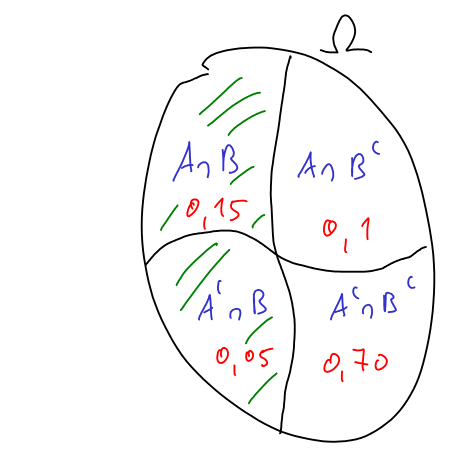
\includegraphics[scale=0.2]{figures/Bedingte Wahrscheinlichkeit.png}
        \end{minipage}
    \end{minipage}
    \\
    Wir wissen, dass $B$ eintritt, also befinden wir uns bereits im Zustandsraum  $\Omega_B := \left \{w\in \Omega \mid  w\in B\right\} $. Ziel ist es also, eine neue Massenfunktion $\mathbb{P}(\cdot |B)$ (auf $\Omega$) zu definieren, die die Information '$\omega\in B$' berücksichtigt. Insbesondere muss also gelten:
    \[
        \mathbb{P}(\omega | B) = 0 \qquad \forall\; \omega\in \Omega_B^{c}
    .\] 
    Zudem wollen wir, dass die Information '$\omega \in B$' dieselbe ist für alle $w\in \Omega_B$, d.h.
    \[
        p(\omega|B) = \subset \cdot p(\omega) \qquad \forall \; \omega\in \Omega_B
    .\] 
    wobei $p(\omega)$ die Massenfunktion von $\mathbb{P}$ ist. Wegen Normierung ergibt sich also bereits
    \[
        1 = \sum_{\omega\in \Omega} \mathbb{P}(\omega|B) = o\cdot \sum_{\omega\in \Omega_B} p(\omega) \quad \iff  \quad c = \frac{1}{\mathbb{P}(B)}
    .\] 
    Also ergibt sich, dass 
    \[
        p(\omega\mid B) = \begin{cases}
            \frac{p(\omega)}{\mathbb{P}(B)} & \text{falls } \omega\in B \\
            0 & \text{sonst}
        \end{cases}
    .\] 
    Wir können das ganze so darstellen: \\
    \begin{minipage}[t]{\textwidth}
        \centering
        \vspace{-2ex}
    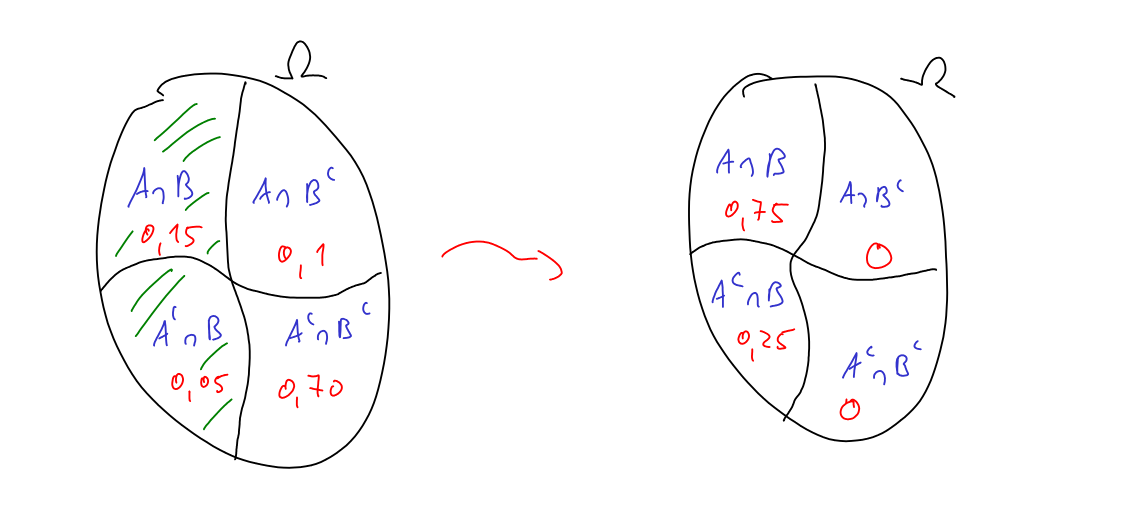
\includegraphics[scale=0.2]{figures/Bedingte Wahrscheinlichkeit II.png}
    \captionof{figure}{Änderung des Zustandsraums bei bedingten Wahrscheinlichkeiten}
    \vspace{2ex}
    \end{minipage}
    Wir erhalten also:
    \begin{answer}
        Ein Kind, das mit 6 Monaten krabbelt, wird mit einer Wahrscheinlichkeit von $75\%$ mit 10 Monaten laufen können.
    \end{answer}
\end{example}
\todo{Besser Skizzen machen}
\begin{definition}[Bedingte Wahrscheinlichkeit]\label{def:bedingte-wahrscheinlichkeit}
    Sei $(\Omega, \mathcal{F}, \mathbb{P})$ ein Wahrscheinlichkeitsraum. Seien $A,B\in \mathcal{F}$ Ereigniss mit $\mathbb{P}(B) \neq  0$. Dann definieren wir
    \[
        \mathbb{P}(A \mid B) := \frac{\mathbb{P}(A\cap B)}{\mathbb{P}(B)}
    .\] 
    und nennen dise die \vocab[Wahrscheinlichkeit!bedingte]{bedingte Wahrscheinlichkeit von $A$ gegeben  $B$}. 
\end{definition}
\begin{remark}
       Die Abbildung
               \begin{equation*}
                   \mathbb{P}(\cdot \mid B): \left| \begin{array}{c c l} 
               \mathcal{F} & \longrightarrow & \R_+ \\
               A & \longmapsto &  \mathbb{P}(A\mid B)
               \end{array} \right.
           \end{equation*}
           ist eine Wahrscheinlichkeitsverteilung auf $(\Omega,\mathcal{F})$, die wir auch die \vocab[Wahrscheinlichkeitsverteilung!bedingte]{bedingte Wahrscheinlichkeitsverteilung gegeben $B$} nennen.
\end{remark}
\begin{definition}[Bedingter Erwartungswert]\label{def:bedingter-erwartungswert}
    Sei $X:\Omega\to \mathcal{S}\subset \R$ eine (diskrete) Zufallsvariable mit Verteilung $\mathbb{P}(\cdot \mid B)$. Dann hat $X$ den Erwartungswert
    \[
        \sum_{s\in \mathcal{S}} s\cdot \mathbb{P}(X = s | B) =: \mathbb{E}(X\mid B)
    .\] 
    Dieser heißt \vocab[Erwartungswert!bedingter]{bedingter Erwartungswert von $X$ gegeben  $B$}. 
\end{definition}
\begin{example}
    Wir werfen eine faire Münze $N$ mal, dabei beobachten wir $n$ mal das Ergebnis 'Zahl'.
     \begin{question}
        Was ist die Wahrscheinlichkeit, dass bei den ersten $m$ Würfen immer 'Zahl' gefallen ist?
    \end{question}
    Ohne Weitere Informationen (dass insgesamt $n$ mal Zahl gefallen ist) würden wir hier $\mathbb{P} \equiv \frac{1}{2^m}$ erhalten. \\
    Betrachte nun den Zustandsraum
    \[
        \Omega = \left \{\omega = (x_1,\ldots,x_N)\mid x_i \in \left \{0,1\right\},1\leq i\leq N \right\} 
    .\] 
    wobei
    \[
    x_k := \begin{cases}
        1 & \text{falls $k$-ter Wurf ist 'Zahl'} \\
        0 & \text{falls $k$-ter Wurf ist 'Kopf'}
    \end{cases}
    .\] 
    und versehe ihn mit $\mathcal{F} = \mathcal{P}(\Omega)$ sowie $\mathbb{P}$ als Gleichverteilung auf $\Omega$. Mit $X_k(\omega) := x_k$ interessieren wir uns also für
    \[
        \mathbb{P}\left(X_1=X_2=\ldots=X_m =1 \mid  \sum_{k=1}^N X_k  =n\right)
    .\]
    Nach Definition ist dies
    \[
        \begin{split}
        &= \frac{\mathbb{P}\left(\left(X_1=\ldots=X_m = 1\right) \cap  \left(\sum\limits_{k=m+1}^N X_k = n-m\right)\right)}{\mathbb{P}\left(\sum\limits_{k=1}^N X_k = n\right)} \\
        &= \frac{\frac{1}{2^N} \binom{N-m}{n-m}}{\frac{1}{2^N}\binom{N}{n}} \\
        &= \frac{(N-m)!}{(n-m)!(N-n)!} \cdot  \frac{(N-n)! n!}{N!} \\
        &= \frac{(N-m)! n!}{N! (n-m)!}
        \end{split}
    .\] 
\end{example}
\begin{notation}
    Zur Vereinfachung der Notation schreiben wir oft
    \[
    \mathbb{P}(X_1=X_2=a) = \mathbb{P}(\left \{\omega\in \Omega \mid  X_1(\omega) = a\right\} \cap \left\{ \omega\in \Omega \mid X_2(\omega) =a\right\} )
    .\] 
    sowie
    \[
    \mathbb{P}(X_1=a, X_2=b) = \mathbb{P}(\left \{\omega\in \Omega \mid  X_1(\omega) = a \right\} \cap \left\{\omega\in \Omega\mid X_2(\omega)  =b\right\} )
    .\] 
\end{notation}
Wir haben gerade aus einer Wahrscheinlichkeitsverteilung $\mathbb{P}$ die Verteilung $\mathbb{P}(\cdot \mid B)$ gewonnen. Das ganze geht auch umgekehrt:
\begin{theorem}\label{thm:zerlegung-in-ereignisse-ergibt-aufaddieren-bedingter-wahrscheinlichkeiten}
    Sei $\Omega = \bigcup_{k\in I} H_k$ eine \emphasize{disjunkte} Zerlegung von $\Omega$ in (abzählbar viele) Ereignisse $H_k, k\in I$, wobei $\mathbb{P}(H_k) \neq 0$. Dann ist $\forall A\in \mathcal{F}$:
    \[
        \mathbb{P}(A) = \sum_{k\in I} \mathbb{P}(A \mid H_k) \cdot \mathbb{P}(H_k)
    .\] 
\end{theorem}
\begin{proof}
    $\forall A\in \mathcal{F}$ ist
    \[
        A= A \cap  \bigcup_{k\in I} H_k = \bigsqcup_{k\in I} (A\cap H_k) 
    .\] 
    eine disjunkte Vereinigung. Also folgt aus $\sigma$-Additivität, dass
    \begin{equation*}
        \begin{split}
            \mathbb{P}(A) &= \sum_{k\in I} \mathbb{P}(A\cap H_k) \\
                          &= \sum_{\substack{ k\in I\\ \mathbb{P}(H_k)\neq 0}} \mathbb{P}(A\cap H_k) \\
                          &=\sum_{\substack{ k\in I \\ \mathbb{P}(H_k)}\neq 0} \mathbb{P}(A\mid H_k) \cdot  \mathbb{P}(H_k)
        \end{split}
    \end{equation*}
\end{proof}
\begin{example}
    Eine Urne $A$ enthält {\color{red} 2 rote} und {\color{blue} 3 blaue} Kugeln. In Urne  $B$ liegen umgekehrt {\color{red} 3 rote} und nur {\color{blue} 2 blaue} Kugeln. Wir gehen davon aus, dass die Urnen immer gut gemischt sind. Nun machen wir Folgendes:
    \begin{enumerate}[label=\protect\circled{\arabic*}]
        \item Wir ziehen eine Kugel $K_1$ aus $A$ und legen sie in  $B$
        \item Wir ziehen eine Kugel  $K_2$ aus $B$ und lg
    \end{enumerate}
    \begin{question}
    Was ist die Wahrscheinlichkeit, dass $K_2$ {\color{red} rot} ist?
    \end{question}
Wir erhalten nun
\[
    \begin{split}
        \mathbb{P}(K_2 \text{ ist rot}) &= \mathbb{P}(K_2 \text{ rot} \mid  K_1 \text{ rot})\cdot \mathbb{P}(K_1 \text{ rot}) \\
                                        &+\mathbb{P}(K_2 \text{ rot}\mid K_1 \text{ blau})\cdot \mathbb{P}(K_1 \text{ blau}) \\
    &= \frac{4}{6}\cdot \frac{2}{5} + \frac{3}{6}\cdot \frac{3}{5} = \frac{17}{30}
    \end{split}
.\] 
\end{example}
\todo{Graphik einfügen}
\subsection{Baye'sche Regel}
In der Baye'schen Statistik ist $\mathbb{P}(H_k)$ auch die \vocab{a-priori-Einschätzung} der Wahrscheinlichkeit einer Hypothese $H_k$, das könnte z.B. sein
\[
    \color{green!50!black} H_k = \{\text{Die Unfallskosten pro Jahr liegen im Bereich } [100k,100(k+1))\}
.\] 
Aus statistischen Daten weiß man, dass ein Ereignis $A\in \mathcal{F}$ mit einer Wahrscheinlichkeit $\mathbb{P}(A) \neq 0$ eintritt, also z.B.
\[
    \color{green!50!black} A = '\text{Es handelt sich um  einen Auffahrunfall}'
.\] 
Dazu kennt man $\mathbb{P}(A\mid H_k)$. Falls $A$ eintritt, werden die Versicherungskosten neu berechnet, auf der Basis von
 \[
     \mathbb{P}(H_k \mid A)
.\] 
Dies nennt man dann auch \vocab{a-posteriori-Verteilung} von $H_k$.
\begin{corollary}[Baye'sche Regel]\label{cor:bayes}
    Für $A\in \mathcal{F}$ mit $\mathbb{P}(A)\neq 0$ gilt
    \[
        \mathbb{P}(H_k \mid A) = \frac{\mathbb{P}(A\mid H_k)\cdot \mathbb{P}(H_k)}{\sum\limits _{\substack{l\in I\\ \mathbb{P}(H_l)\neq 0}} \mathbb{P}(A\mid H_l)\cdot \mathbb{P}(H_l)}
    .\] 
\end{corollary}
\begin{proof}
    Es ist
    \[
        \mathbb{P}(H_k \mid A) = \frac{\mathbb{P}(H_k \cap A)}{\mathbb{P}(A)} =\frac{\mathbb{P}(A\mid H_k)\cdot \mathbb{P}(H_kr}{\mathbb{P}(A)}
    .\] 
    Aus \autoref{thm:zerlegung-in-ereignisse-ergibt-aufaddieren-bedingter-wahrscheinlichkeiten} erhalten wir nun aber genau
    \[
        \mathbb{P}(A) = \sum_{\substack{l\in I \\ \mathbb{P}(H_l)\neq 0} } \mathbb{P}(A\mid H_l)\cdot \mathbb{P}(H_l)
    .\] 
    und wir sind fertig.
\end{proof}
\begin{example}
    Eine Krankheit $K$ tritt selten auf, mit einer Häufigkeit von  $10^{-4}$, also bei 10 von 100.000 Menschen. Ein Test zur Erkennung der Krankheit ist positiv (+) bei $96\%$ der Kranken und  $0,1\%$ der Gesunden. \\
    Der Test liefert also  $0,1\%$ falsch positive und  $4\%$ falsch negative Ergebnisse.
     \begin{question}
        Was ist die Wahrscheinlichkeit, dass jemand krank ist, sofern er positiv getesten wurde?
    \end{question}
    \begin{itemize}
        \item Die \emphasize{a-priori-Wahrscheinlichkeit} beträgt $\mathbb{P}(k) = 10^{-4}$ sowie $\mathbb{P}(K^{c}) = 1-10^{-4}$.
        \item Wir kennen die \emphasize{bedingten Wahrscheinlichkeiten} $\mathbb{P}(+\mid K) = 0,96$ sowie $\mathbb{P}(+\mid K^{c}) = 0,001$.
        \item Als \emphasize{A-posteriori Wahrscheinlichkeit} erhalten wir nun:
            \begin{equation*}
                \begin{split}
                    \mathbb{P}(K\mid +) &= \frac{\mathbb{P}(+\mid K)\cdot \mathbb{P}(K)}{\mathbb{P}(+ \mid  K) \cdot \mathbb{P}(K) + \mathbb{P}(+ \mid K^{c}) \cdot  \mathbb{P}(K^{c})} \\
                                        &= \frac{0,96 \cdot 10^{-4}}{0,96\cdot 10^{-4}+0,001\cdot (1-10^{-4})} \\
                                        &\approx 9,6\%
                \end{split}
            \end{equation*}
    \end{itemize}
    \begin{answer}
        \color{blue} Die Wahrscheinlichkeit, dass man krank ist, wenn man positiv getestet ist, beträgt also (nur) $9,6\%$.
    \end{answer}
\end{example}
\begin{remark*}
    Ein Test hat üblicherweise eine Sensitivität und ein Spezifität. Die Sensitivität gibt an, welcher Anteil der tatsächlich infizierten positiv getestet werden. Die Spezifität gibt an, welcher Anteil der gesunden Menschen auch negativ gestetest wird.
\end{remark*}
\begin{example}[Aktuelle Corona-Zahlen]
    Bei den aktuellen Schnelltestes gibt es (in etwa) eine falsch-positiven Rate von $2\%$, also  $\mathbb{P}(B\mid K^{c}) = 2\%$, und eine falsch-negativen Rate von $20\%$, also  $\mathbb{P}(-\mid K) = 20\%$. \\
    Bei einer Inzidenz von 150-200 pro 100.000 Einwohner pro Woche, einer Dunkelziffer nah bei 2 ergibt sich eine Schätzung der aktuell infizierten von
    \[
        \mathbb{P}(K) \in [0.005, 0.01]
    .\] 
    (Zum Vergleich: Die aktuell gemeldeten positiven Fälle liegen bei $0,0035$). \\
    Nun können wir wieder berechnen:
    \[
                \begin{split}
                    \mathbb{P}(K\mid +) &= \frac{\mathbb{P}(+\mid K)\cdot \mathbb{P}(K)}{\mathbb{P}(+ \mid  K) \cdot \mathbb{P}(K) + \mathbb{P}(+ \mid K^{c}) \cdot  \mathbb{P}(K^{c})} \\
                                        &= \frac{0,8\cdot \mathbb{P}(K)}{0,8 \mathbb{P}(K) + 0,02 (1-\mathbb{P}(K)}
                \end{split}
            \]
            Wir erhalten
            \begin{enumerate}[label=\protect\circled{\alph*}]
                \item Mit $\mathbb{P}(K) = 0,005$ eine Wahrscheinlichkeit von $\mathbb{P}(K\mid +) \approx 17\%$
                \item Mit $\mathbb{P}(K) = 0,01$ eine Wahrscheinlichkeit von $\mathbb{P}(K\mid +) \approx 29\%$ 
                \item Mit $\mathbb{P}(K) = 0,001$ eine Wahrscheinlichkeit von $\mathbb{P}(K\mid +) \approx 3,8\%$
            \end{enumerate}
            \begin{question}
                Lohnt es sich die Schnelltests in den Schulen zu machen? Also: Was ist $\mathbb{P}(K\mid -)$
            \end{question}
            Auch das lässt sich mit der gleichen Formel beantworten, mit $\mathbb{P}(-\mid K) = 0,2$ und $\mathbb{P}(-\mid K^{c})=0,98$ erhalten wir
            \begin{enumerate}[label=\protect\circled{\alph*}]
                \item Für $\mathbb{P}(K) = 0,005$ eine Wahrscheinlichkeit von $\mathbb{P}(K\mid -) \approx 0,1\%$
                \item Für $\mathbb{P}(K) = 0,01 $ eine Wahrscheinlichkeit von $\mathbb{P}(K\mid -) \approx 0,2\%$
                \item Für $\mathbb{P}(K) = 0,001$ eine Wahrscheinlichkeit von $\mathbb{P}(K\mid -) \approx 0,02\%$
            \end{enumerate}
\end{example}













    \lecture[Mehrstufie Modelle. Produktmodelle.]{Mi 05 Mai 2021 10:11}{Mehrstufige Modelle}
\subsection{Mehrstufige Modelle}
Sei eine Folge von $n$ Zufallsexperimenten in den Wahrscheinlichkeitsräumen  $\Omega_1,\Omega_2,\ldots,\Omega_n$ gegeben. Wir definieren ein \vocab{$n$-stufiges Zufallsexperiment} durch
\begin{itemize}
    \item $\Omega = \Omega_1\times \Omega_2\times \ldots\times \Omega_n = \left \{\omega=(\omega_1,\ldots,\omega_n) \mid  \omega_k \in \Omega_k, 1\leq k\leq n\right\} $ 
    \item $\mathcal{F} = \mathcal{P}(\Omega)$.
    \item Definiere die Zufallsvariablen
        \[
            X_k(\omega) = \omega_k \qquad 1\leq k\leq n
        .\] 
        Den Index $k$ interpretieren wir hierbei als Zeit.  $k \mapsto  X_k$ ist eine Trajektion von $X = (X_1,\ldots,X_n)$ ?
    \item $\mathbb{P}=?$. Wir konstruieren $\mathbb{P}$ auf $(\Omega,\mathcal{F})$ mit
        \begin{enumerate}[label=\protect\circled{\alph*}]
            \item Der Anfangsverteilung $\mathbb{P}(X_1=x_1) := p_1(x_1)$ für alle $x_1\in \Omega_1$.
            \item Den bedingten Verteilungen
                 \[
                     \mathbb{P}(X_k = x_k \mid  X_1 = x_1, X_2 = x_2, \ldots, X_{k-1} = x_{k-1}) =: p_k(x_k\mid x_1,\ldots,x_{k-1})
                .\] 
                für alle $x_l\in \Omega_l$, $1\leq l\leq k-1$, sodass $\mathbb{P}(X_1=x_1,\ldots,X_{k-1}=x_{k-1})\neq 0$.
        \end{enumerate}
\end{itemize}i
\begin{remark*}
    Man kann das Allgemeiner machen, indem wir $\mathcal{F}$ als die Produktsigmalalgebra der $\mathcal{F}_i$ wählen.
\end{remark*}
\begin{theorem}\label{thm:stufenmodell}
    Sei $p_i(\cdot )$ die Massenfunktion einer Wahrscheinlichkeitsverteilung auf $\Omega_i$ und $p_k(\cdot \mid x_1,\ldots,x_{k-1})$ für alle $1\leq k\leq n$ mit $x_1\in \Omega_1, \ldots,x_{k-1} \in \Omega_{k-1}$ eine Massenfunktion auf $\Omega_k$. \\
    Dann existiert eine eindeutige Wahrscheinlichkeitsverteilung $\mathbb{P}$ auf $(\Omega,\mathcal{F})$, sodass
    \begin{enumerate}[label=\protect\circled{\alph*}]
        \item $\mathbb{P}(X_1=x_1) = p_1(x_1) \quad \forall x_1\in \Omega_1$
        \item $\mathbb{P}(X_k = x_k) \mid  X_1 = x_1,\ldots,X_{k-1}=x_{k-1}) = p_k(x_k \mid  x_1,\ldots,x_{k-1})$
    \end{enumerate}
    Die Wahrscheinlichkeitsverteilung $\mathbb{P}$ hat die Massenfunktion
    \[
        p(x_1,\ldots,x_n) = p_1(x_1) p_2(x_2\mid x_1) \cdot \ldots\cdot p_n(x_n \mid x_1,\ldots, x_{n-1})
    .\] 
\end{theorem}
\begin{proof}
    \begin{enumerate}[1)]
        \item Nimm zunächst an, dass solch ein Maß existiert, wir zeigen die letzte Aussage. Sei $\mathbb{P}$ sodass \circled{a} und \circled{b} erfüllt sind. Dann ist
             \[
                 \forall 1\leq k\leq n \colon \mathbb{P}(X_1=x_1,\ldots,X_k=x_k) = p(x_1,\ldots,x_k)
            .\] 
            \begin{itemize}
                \item Für $k=1$ gilt das (aus \circled{a}).
                \item Falls es für $k-1$ gilt, so haben wir die Fälle
                \item  $p(x_1,\ldots,x_{k-1})=0$, dann ist $0=0$ wahr.
                \item Falls $p(x_1,\ldots,x_{k-1})\neq 0$, so ist
                    \[
                        \begin{split}
                        &\; \mathbb{P}(X_1=x_1,\ldots,X_k=x_k) \\
                        &= \mathbb{P}(X_k = x_k \mid  X_1 = x_1, \ldots, X_{k-1} = x_{k-1})\cdot \mathbb{P}(X_1=x_1, \ldots, X_{k-1} = x_{k-1}) \\
                        &= p_1(x_1)\cdot \ldots p_{k-1}(x_{k-1}\mid x_1,\ldots,x_{k-2}r\cdot p_k(x_k\mid x_1,\ldots,x_{k-1}) = p(x_1,\ldots,x_k)
                        \end{split}
                    .\] 
            \end{itemize}
    \end{enumerate}
    Normierung: $\forall x\in \Omega, x = (x_1,\ldots,x_n)$ mit $x_k \in \Omega_k$ ist
    \[
        \begin{split}
            \sum_{x\in \Omega} p(x) &= \sum_{x_1\in \Omega_1} \ldots \sum_{x_n \in \Omega_n} p(x_1,\ldots.,x_n) \\
                                    &= \sum_{x_1\in \Omega_1} p(x_1) \sum_{x_2\in \Omega_2} p(x_2\mid x_1) \ldots \sum_{x_n \in \Omega_n} p(x_n \mid  x_1,\ldots,x_{n-1}) = 1
        \end{split}
    .\] 
    Für Eigenschaft \circled{b} ist
    \begin{equation*}
        \begin{split}
            \mathbb{P}(X_1&=x_1,\ldots,X_k=x_k) = \sum_{x_{k+1}\in \Omega_{k+1}} \ldots \sum_{x_n \in \Omega_n} p(x_1,\ldots,x_n) \\
                          &= p_1(x_1)\ldots p_{k-1}(x_{k-1}\mid  x_1,\ldots,x_{k-2}) p_k(x_k \mid  x_1,\ldots,x_{k-1}) \\
                          &= \mathbb{P}(X_1=x_1,\ldots,X_{k-1}=x_{k-1})p_k(x_k \mid  x_1,\ldots,x_{k-1})
        \end{split}
    \end{equation*}
    Also erhalten wir
    \[
        \mathbb{P}(X_k = x_k \mid  X_1 = x_1,\ldots,X_{k-1} = x_{k-1}) = p_k(x_k \mid  x_1,\ldots,x_{k-1})
    .\] 
\end{proof}
\todo{Beweis nochmal sortieren}
\begin{note}
    Mir ist noch nicht klar, wo wir im Beweis des Satzes jetzt gezeigt haben wollen, dass solch ein Wahrscheinlichkeitsmaß existiert, das muss ich noch ausarbeiten.
\end{note}
\begin{remark}
    Falls $p_k(x_k \mid  x_1,\ldots,x_{k-1})$ nur eine Funktion von $x_{k-1},\ldots,x_{k-m-1}$, dann sagen wir, dass unser Modell ein Gedächtnis von $m$ Schritten hat.
\end{remark}

\subsubsection{Produktmodelle}
Falls $p_k(x_k \mid  x_1 = \ldots = x_{k-1}) = p_k(x_k)$, d.h. $x_k$ hängt nicht von den Werten  $x_1,\ldots,x_{k-1}$ ab. Dann erhalten wir aus \autoref{thm:stufenmodell}, dass
\[
    p(x_1,\ldots,x_n) = \prod_{k=1}^n p_k(x_k)
.\] 

\begin{definition}[Produktmodell]\label{def:produktmodell}
    Die Wahrscheinlichkeitsverteilung $\mathbb{P}$ auf $\Omega = \Omega_1\times \ldots\times \Omega_n$ mit Massenfunktion
    \[
        p(x_1,\ldots,x_n) = \prod_{k=1}^n p_k(x_k)
    .\] 
    heißt \vocab{Produkt von $\mathbb{P}_1,\ldots,\mathbb{P}_n$}. ($\mathbb{P}_k$ hat Massenfunktion $p_k$).
\end{definition}
\begin{notation}
    Wir schreiben $\mathbb{P} = \mathbb{P} \otimes \mathbb{P}_2 \otimes \ldots\otimes  \mathbb{P}_n$, wenn $\mathbb{P}$ das Produkt von $\mathbb{P}_1,\ldots,\mathbb{P}_n$ ist.
\end{notation}
\begin{example}
    Seien $n$ unabhängige  0-1-Experimente mit Erfolgswahrscheinlichkeit  $p$ gegeben. Also
     \[
    \Omega_1=\ldots=\Omega_n =\left \{0,1\right\} 
    .\] 
    und $p_k(1) = p = 1-p_k(0)$ für  $k=1,\ldots,n$. dann ist $p_k(x) = (1-p)\left( \frac{p}{1-p} \right) ^x$ für $x\in \left \{0,1\right\} $. Die entstehende Verteilung
    \[
        p(x_1,\ldots,x_n) = (1-p)^n \prod_{k=1}^n \left( \frac{p}{1-p} \right) ^{x_k}
    .\] 
    ist die \vocab{$n$-dimensionale Bernoulli-Verteilung mit Parameter  $p$ }.
\end{example}
\begin{theorem}
    Sei $(\Omega, \mathcal{F}, \mathbb{P})$ ein Produktmodell. Dann ist für beliebige Ereignisse $A_k \subset \Omega_k$, $k=1,\ldots,n$:
    \[
        \mathbb{P}(A_1\times \ldots\times A_n ) = \prod_{k=1}^n \mathbb{P}_k(A_k)
    .\] 
    und $\mathbb{P}(\tilde{A}_k) = \mathbb{P}_k(A_k)$, wobei
    \[
    \tilde{A}_k := \Omega_1\times \ldots\times \Omega_{k-1}\times A_k \times \Omega_{k+1} \times \ldots\times \Omega_n
    .\] 
    Deswegen sind $\tilde{A}_1,\ldots,\tilde{A}_n$ unabhängige Ereignisse.
\end{theorem}
\begin{proof}
    Es ist
    \begin{equation*}
        \begin{split}
            \mathbb{P}(A_1\times \ldots\times A_n) &= \mathbb{P}((X_1,\ldots,X_n)\in A_1\times \ldots\times A_n))  \\
                                                   &= \sum_{(x_1,\ldots,x_n) \in A_1\times \ldots\times A_n} p(x_1,\ldots,x_n) \\
                                                   &= \sum_{x_1\in A_1} \ldots\sum_{x_n\in A_n} p_1(x_1)\cdot \ldots p_n(x_n) \\
                                                   &=\prod_{k=1}^n \sum_{x_k\in A_k} p_k(a_k) \\
                                                   &= \prod_{k=1}^n \mathbb{P}(A_k)
        \end{split}
    \end{equation*}
    Es ergibt sich leicht
    \begin{IEEEeqnarray*}{rCl}
        \mathbb{P}(\tilde{A}_k) &=& \mathbb{P}(X_k \in A_k, X_l \in \Omega_l \; \forall l\neq k) \\
                                & = & \left( \prod_{l\neq k}\underbrace{ \mathbb{P}_l(X_l \in \Omega_l) }_{=1} \right)\cdot \mathbb{P}_k(X_k\in A_k) \\
                                & = & \mathbb{P}k(A_k)
    \end{IEEEeqnarray*}
    Damit ergibt sich schlussendlich für beliebiges $I = \left \{i_1,\ldots,i_l\right\}$:
    \begin{IEEEeqnarray*}{rCl}
    \mathbb{P}(\tilde{A}_{i_1} \cap  \ldots \cap \tilde{A}_{i_l}) & = & \mathbb{P}\left(\bigcap_{i \in  I} \left \{X_i \in A_i\right\} \cap \bigcap_{j\neq I} \left \{x_j \in \Omega_j\right\} \right) \\
                                                                  & = & \prod_{i\in I} \mathbb{P}_i(A_i) \cdot  \prod_{j\neq I} \underbrace{\mathbb{P}_j(\Omega_j)}_{=1} \\
                                                                  & = & \prod_{i \in I}\mathbb{P}_i(A_i) \\
                                                                  & \stackrel{\mathbb{P}(A_i) = \mathbb{P}(\tilde{A}_i)}{=} & \prod_{k=1}^l \mathbb{P}(\tilde{A}_{i_k})
    \end{IEEEeqnarray*}
    
    
\end{proof}
\begin{remark}
    \begin{itemize}
        \item Es ist $\Omega = \Omega_1\times \ldots\times \Omega_n$
        \item Eigentlich müssen wir $(\Omega_i, \mathcal{F}_i, \mathbb{P}_i)$ als entsprechende Wahrscheinlichkeitsräume betrachten, wir unterdrücken aber oft die Notation $\mathcal{F}_i, \mathbb{P}_i$
    \end{itemize}
Im Allgemeinen setzen wir 
\[
\mathcal{F} = \mathcal{F}_1 \otimes \ldots\otimes \mathcal{F}_n
.\] 
wobei $\mathcal{F}$ dann die $\sigma$-Algebra ist, die von  $A_1\times \ldots\times A_n$ mit $A_i \in \mathcal{F}_i$ erzeugt ist. Im Spezialfall $F_i = \mathcal{P}(\Omega_i)$ ergibt sich insbesondere wieder der uns bekannte Fall $\mathcal{F} = \mathcal{P}(\Omega)$. \\
Für Produktmodelle erhalten wir also $\Omega = \Omega_1\times \ldots\times \Omega_n$, $\mathcal{F} = \mathcal{F}_1 \otimes  \ldots \otimes  \mathcal{F}_n$ sowie $\mathbb{P} = \mathbb{P}_1 \otimes  \ldots \otimes  \mathbb{P}_n$. \\
Beachte, dass $\mathcal{F}_1 \otimes  \ldots \otimes  \mathcal{F}_n \neq  \mathcal{F}_1 \times  \ldots \times  \mathcal{F}_n$ im Allgemeinen, wie das folgende Beispiel zeigt.
\end{remark}
\begin{example}
    Im Fall $n=2$ ergibt sich Beispielsweise folgende Situation:
     \begin{tikzpicture}
         \draw[->] (-0.5,0) -- (5,0);
         \draw[->] (0,-0.5) -- (0,5);
         \coordinate (A1) at (2,3);
         \coordinate (A2) at (4,4.5);
         \draw (A1) -- (A1) -| (A2) node[anchor = west] {$A_1\times A_2$} -- (A2) -- (A2) -| (A1) -- (A1);
         \coordinate (B1) at (1,1);
         \coordinate (B2) at (3,4);
         \draw (B1) node [anchor = north] {$B_1\times B_2$}-- (B1) -| (B2)  -- (B2) -- (B2) -| (B1) -- (B1);
    \end{tikzpicture}
\end{example}



    \lecture[]{Mo 10 Mai 2021 10:15}{}

    \lecture[]{Mi 12 Mai 2021 10:16}{}
\begin{example}
    Sei $\mathcal{S} = \left \{0,1\right\}$ und $α,β\in (0,1)$. Setze
    \[
        P = \begin{pmatrix} 1 - α & α \\ β & 1-β \end{pmatrix} 
    .\] 
    Oft machen wir eine graphische Darstellung:
    Wir wollen also $P^n$ ausrechnen, um das Verhalten der Markovkette zu studieren. 
     \begin{enumerate}[label=\protect\circled{\alph*}]
        \item Man könnte nun $P$ diagonalisieren, also  $P = U \Lambda U^{-1}$, wobei $A$ Diagonalform hat, so ist $P^n = U \Lambda ^n U^{-1}$, und die Potenzen von $\Lambda$ können wir leicht berechnen.
        \item  $P^n$ ist stochastisch, also ist auch  $P^n(0,0) + P^n(0,1)=1$,  $P^n(1,1) + P^n(1,0) = 1$, weil  $P^n$ stochastisch ist. Wir wollen uns nun, welchen Wert $P^n(0,0)$ hat, dazu machen wir den Rekursion Ansatz:
            \begin{itemize}
                \item Sind wir nach $n-1$ Schritten wieder bei der  $0$, so müssen wir von  $0$ nach  $0$ gehen
                \item Sind wir nach  $n-1$ Schritten bei der  $1$, so müssen wir im  $n$-ten von  $1$ nach  $0$ gehen
            \end{itemize}
            Also ergibt sich
            \begin{IEEEeqnarray*}{rCl}
                P^n(0,0) &=& P^{n-1}(0,0)\cdot P(0,0) + P^{n-1}(0,1) \cdot P(1,0)  \\
                         & = & P^{n-1}(0,0)(1-α)+ \underbrace{P^{n-1}(0,1)}_{= 1-P^{n-1}(0,0)}\cdot β \\
                         & = & P^{n-1}(0,0)(1-α-β) + β
            \end{IEEEeqnarray*}
            Als Rekursion suhcne wir also eine Funktion $n \mapsto f(n)$, sodass
             \[
            \begin{cases}
                f(n) & = β + (1-α-β) f(n-1) \\
                f(1) & = 1-α
            \end{cases}
            .\] 
            Als Lösung ergibt sich (Theorie der linearen Rekursionen!):
            \[
                f(n) = \frac{β}{α+β} + \frac{α}{α+β}(1-α-β)^n
            .\] 
            Damit ergibt sich
            \[
                P^n = \begin{pmatrix} \frac{β}{α+β} & \frac{α}{α+β} \\ \frac{β}{α+β} & \frac{α}{α+β} \end{pmatrix}  + (1-α-β)^n \begin{pmatrix} \frac{α}{α+β} & \frac{-α }{\alpha + \beta} \\ \frac{-\beta }{\alpha + \beta} & \frac{\beta}{\alpha + \beta} \end{pmatrix} 
            .\] 
            Wir beschränken uns auf $α,β \in (0,1)$. Da $(1-α-β)^n \to 0$ exponentiell schnell, ergibt sich
            \[
            \lim_{n \to \infty} P^n = \begin{pmatrix} \frac{β}{α+β} & \frac{α}{α+β} \\ \frac{β}{α+β} & \frac{α}{α+β} \end{pmatrix} 
            .\] 
            Wir stellen fest, dass diese Matrix Rang 1 hat. Ebenso ergibt sich
\[
\lim_{n \to \infty} \mu_0 P^n = \begin{pmatrix} \frac{β}{α+β}, \frac{α}{α+β} \end{pmatrix} 
.\] 
und dieser ist von $μ_0$ unabhängig.
    \end{enumerate}
\end{example}
\todo{Grafik}
\subsection{Unabhängige Zufallsvariablen}
\subsubsection{Unabhängige Ereignisse}

\begin{definition}[Unabhängigkeit]\label{def:unabhängigkeit-von-ereignissen}
    Eine Familie von Ereignissen $\left \{A_k\right\} _{k \in I}$ heißt unabhängig, falls 
    \[
        P(A_{i_1}\cap \ldots\cap A_{i_n}) = \prod_{k=1}^n P(A_{i_k})
    .\] 
    für alle verschiedenen $i_{1},\ldots.i_{n}\in I$ und für alle $n\leq \abs{I}$.
\end{definition}
Seien $A,B\in \mathcal{F}$, sodass $\mathbb{P}(A) \neq  0, \mathbb{P}(B) \neq 0$. Dann sind $A$ und  $B$ unabhängig gwd
 \[
     \mathbb{P}(A\mid B) = \mathbb{P}(A) \iff  \mathbb{P}(B\mid A) = \mathbb{P}(B)
.\]
\begin{warning}
    Falls $\mathbb{P}(A_i \cap  A_j) = \mathbb{P}(A_i) \cdot \mathbb{P}(A_j)$ für $i\neq j \in I$, so folgt noch nicht, dass $\left \{A_i\right\} _{i \in I}$ unabhängig ist!
\end{warning}
\begin{example}
    Betrachte 3 faire Münzen, also
    \[
        \Omega = \left \{0,1\right\} ^3 f \left \{(\omega_1,\omega_2,\omega_3) \mid  \omega_i \in  \left \{0,1\right\} \text{ für } i=1,2,3,\right\} 
    .\] 
    wobei 
    \[
    \omega_i = \begin{cases}
        0 & \text{Münze $i$ ist Kopf} \\
        1 & \text{Münze $i$ ist Zahl}
    \end{cases}
    .\] 
    Wir setzen $\mathcal{F} = \mathcal{P}(\Omega)$ und $\mathbb{P}$ als die Gleichverteilung und betrachten die Ereignisse
    \[
    A_1 = \left \{\omega_1 = \omega_2\right\} \qquad A_2 = \left \{\omega_2 = \omega_3\right\}  \qquad A_3 = \left \{\omega_3 = \omega_1\right\} 
    .\] 
    und erhalten unmittelbar
     \[
         \mathbb{P}(A_i) = \frac{4}{8}=\frac{1}{2} \qquad \mathbb{P}(A_i \cap A_j) = \frac{2}{8} = \frac{1}{4} = \mathbb{P}(A_i)\cdot \mathbb{P}(A_j) \; \forall i\neq j
    .\] 
    allerdings ist auch
    \[
        \mathbb{P}(A_1\cap A_2\cap A_3) = \frac{2}{8} \neq  \mathbb{P}(A_1) \mathbb{P}(A_2) \mathbb{P}(A_3)
    .\] 
    also sind die Ereignisse nicht unabhängig, allerdings paarweise unabhängig. Dies liegt daran, dass $A_1 \land A_2 \implies A_3$ etc.
\end{example}
\subsubsection{Unabhängige Zufallsvariablen}

\begin{definition}[Gemeinsame Verteilung]\label{def:gemeinsame-verteilung}
    Seien $X_k : \Omega\to \mathcal{S}_k$ für $1\neq k\leq n$ diskeret Zufallsvariablen auf $(\Omega,\mathcal{F},\mathbb{P})$. Die Verteilung $\mu_{X_1,\ldots,X_n}$ der Zufallsvektoren $(X_1,\ldots,X_n)$ mit Massenfunktion
    \[
        p_{X_1,\ldots,X_n}(a_1,\ldots,a_n) := \mathbb{P}(X_1 = a_1, \ldots, X_n = a_n)
    .\] 
    heißt die \vocab{gemeinsame Verteilung} von $X_1,\ldots,X_n$. 
\end{definition}

\begin{definition}[Unabhängigkeit]\label{def:unabhängigkeit}
    Die diskreten Zufallsvariablen $X_1,\ldots,X_n$ heißen \vocab{unabhängig}, falls
    \[
        \mathbb{P}(X_1=a_1,\ldots,X_n = a_n) = \prod_{k=1}^n \mathbb{P}(X_k = a_k)
    .\]
    für alle $a_1\in \mathcal{S}_1\ldots,a_n \in \mathcal{S}_n$.
\end{definition}

    %! TEX root = ./master.tex
\lecture[]{Mo 17 Mai 2021 10:15}{}

\subsubsection{Abschätzung von Abweichungen}
Seien $X_1,X_2,\ldots,X_n\sim \Ber(p)$ unabhängige Zufallsvariablen. wobei $p\neq 0,1$. Dann ist $\mathcal{S}_n \coloneqq  X_1 + \ldots + X_n \sim  \Bin(n,p)$. Bekannt ist für uns bereits
       \[
            \mathbb{E}\left( \frac{\mathcal{S}_n}{n} \right) = p, \Var\left( \frac{\mathcal{S}_n}{n} \right) = \frac{1}{n^2} \Var(\mathcal{S}_n) = \frac{np(1-p)}{n^2} = \frac{p(1-p)}{n}
        .\] 
        \missingfigure{Binomialverteilung für große $n$}
\begin{question}
    Was ist $\mathbb{P}\left( \abs{\frac{\mathcal{S}_n}{n} -p}\geq ε \right) $, bzw ist das $\leq  ?$ für $n\gg 1$.
\end{question}
\begin{theorem}[Ungleichung von Tchebishev]
    Sei $X$ eine Zufallsvariable auf  $(\Omega,\mathcal{F},\mathbb{P})$. Dann gilt $\forall  ε>0$:
    \[
        \mathbb{P}\left( \abs{X - \mathbb{E}(X)} \geq ε \right) \leq  \frac{\Var(X)}{ε^2}
    .\] 
\end{theorem}
\begin{proof}
    Wir stellen fest, dass beide Seiten unabhängig vom Milltwert sind, also können wir $\mathbb{E}(X) = 0$ voraussetzen, indem wir $Y\coloneqq  X - \mathbb{E}(X)$ als Zufallsvariable betrachten. Wir überlegen uns nun:
    \begin{IEEEeqnarray*}{rCl}
        \mathbb{P}(\abs{X} \geq ε) &=& \mathbb{E}\left( \One_{\abs{X} \geq  ε } \right)  \\
                                   & \stackrel{\leq}{(1)}  & \mathbb{E}\left( \One_{\abs{X} \geq  ε } \frac{X^2}{ε^2}\right) \\
                                   & \leq  & \frac{\mathbb{E}(X^2)}{ε^2} \\
                                   & = & \frac{\Var(X)}{ε^2}
    \end{IEEEeqnarray*}
    Man beachte, dass wir hier bei (1) einfach benutzen, dass $1 \leq  \frac{X^2}{ε^2}$, denn $\abs{X} \geq  ε $.
\end{proof}
Wir lernen nun eine Verallgemeinerung kennen:
\begin{lemma}\label{lm:markov-ungleichung-allgemeiner}
    Sei $X$ enie Zufallsvariable,  $f: \R \to  \R_{+}$ eine \emphasize{monoton wachsende} Zufallsvariable. Dann ist
    \[
        \mathbb{P}(X \geq  a) \leq  \frac{\mathbb{E}(f(X))}{f(a)} \qquad \forall a\in \R
    .\] 
\end{lemma}

\begin{proof}
    Völlig analog:
    \begin{IEEEeqnarray*}{rCl}
        \mathbb{P}(X \geq a) &=& \mathbb{E}(\One_{X\geq a}) \\
                             & \leq  & \mathbb{E}\left( \One_{X\geq a} \frac{f(X)}{f(a)} \right) \\
                             & \leq  & \frac{1}{f(a)} \mathbb{E}(f(X))
    \end{IEEEeqnarray*}
\end{proof}

\begin{example}
    Wir erhalten zum Beispiel die \vocab{Markov-Ungleichung}:
    \[
        \mathbb{P}(\abs{X} \geq ε) \leq  \frac{\mathbb{E}(\abs{X}) }{ε}
    .\] 
\end{example}

\begin{corollary}
    Sei $X$ eine Zufallsvariable auf  $(\Omega,\mathcal{F},\mathbb{P})$. Dann ist
    \[
        \mathbb{P}(X \geq  a) \leq  \inf_{λ\geq 0} e^{-λa} \mathbb{E}(e^{λx})
    .\] 
\end{corollary}

\begin{proof}
    Verwende das Lemma mit $f(x) = e^{λx}$ für alle $λ\geq 0$, dann sind wir schon fertig.
\end{proof}

\begin{theorem}
    Betrachte wieder das Setting zu Beginn des Kapitels. Für alle $ε>0$ ist
     \[
         \mathbb{P}\left( \frac{\mathcal{S}_n}{n}\geq p + ε \right) \leq e^{-cε^2n}
    .\] 
    und
    \[
        \mathbb{P}\left( \frac{\mathcal{S}_n}{n}\leq p-ε \right) \leq  e^{-cε^2n}
    .\] 
    für ein $0<c = c(p)$, das nur von  $p$ abhängt. Also ist
     \[
         \mathbb{P}\left( \abs{\frac{\mathcal{S}_n}{n}-p} \geq  ε  \right)  \leq  2\cdot e^{-cε^2n}
    .\] 
\end{theorem}
\begin{remark}
    Man kann $c= 2$ zeigen.
\end{remark}
    Die Abschätzung konvergiert gegen $0$ exponentiell schnell in  $n$ für  $n\to \infty$.
Wäs würden wir mit Tchebishev erhalten?
\[
    \mathbb{P}\left( \abs{\frac{\mathcal{S}_n}{n}-p} \geq ε \right)  \leq  \frac{1}{ε^2} \Var\left( \frac{\mathcal{S}_n}{n} \right)  = \frac{p(1-p)}{n\cdot ε^2}
.\] 
Das geht auch gegen $0$, aber eben nicht exponentiell (sondern nur quadratisch / polynomiell), also nicht wirklich schnell.
\begin{remark}
    Es gilt sogar
    \[
        \mathbb{P}\left( \abs{\frac{\mathcal{S}_n}{n}-p} \geq \frac{X}{\sqrt{n} } \right) \to 2\cdot \frac{1}{2 \pi \gamma^2} \int_{x}^{\infty} e^{-y^2 / (2σ^2)} \dy
    .\] 
    aber das soll nicht Teil dieser Vorlesung sein.
\end{remark}
\begin{proof}
    Stellen wir zunächst fest, dass wir mit $X \coloneqq  \frac{\mathcal{S}_n}{n}-p$
    \begin{IEEEeqnarray*}{rCl}
        \mathbb{P}\left( \frac{\mathcal{S}_n}{n}\geq p + ε \right)  &=& \mathbb{P}(X \geq  ε)  \\
                                                                    & \leq  & \inf_{λ>0} e^{-λε} \mathbb{E}\left( e^{λ\left( \frac{\mathcal{S}_n}{n}-p \right) } \right) \\
                                                                    & \stackrel{λ\coloneqq  μn}{=}& \inf_{μ> 0} e^{-μn(p+ε)} \underbrace{\mathbb{E}(e^{μ\mathcal{S}_n})}_{= \psi (e^{μ})} \\
    \end{IEEEeqnarray*}
    Setzen wir nun $\psi (z) = \sum_{k=0}^n \binom{n}{k} p^k (1-p)^{n-k}z^k = (p\cdot z + 1-p)^n$, so erhalten wir weiter:
    \begin{IEEEeqnarray*}{rCl}
        \mathbb{P}\left( \frac{\mathcal{S}_n}{n}\geq p+ε \right)         & = & \inf_{μ>0} e^{-n [\underbrace{μ(p+ε) - \ln [p e^{μ} + 1-p]}_{\coloneqq  I(μ,p)}]} 
    \end{IEEEeqnarray*}
    Wir untersuchen nun $I(μ,p)$ weiter:
     \begin{itemize}
         \item $I(0,p) = 0$
         \item  $\frac{d}{d\mu}I(μ,p) = p + ε - \frac{pe^{μ}}{1-p + p e^{μ}}$ und diese ist 0 genau dann, wenn $e ^{ μ} = \frac{(1-p) (p+ε)}{p(1-p-ε)} =: e^{μ^*}$ 
         \item Es ist
                 \begin{IEEEeqnarray*}{rCl}
                     I(μ^*,p) &=& (p+ε) \ln \left( \frac{p+ε}{p} \right)  + (1-p-ε) \ln \left( \frac{1-p-ε}{} \right) \\
                              & \stackrel{\text{Taylor}}{=} & \frac{ε^2}{2p(1-p)} + O(ε^3)
                 \end{IEEEeqnarray*}
                 Also erhalten wir für kleine $ε$ und  $p\in (0,1)$, dass 
                 \[
                     I(μ^*,p) \geq  2 ε^2 + O(ε^3) \geq  ε^2
                 .\] 
                 und damit
                 \[
                     \mathbb{P}\left( \frac{\mathcal{S}_n}{n}\geq p+ ε \right) \leq  e^{-nε^2}
                 .\] 
                 Setze nun $X = -\frac{\mathcal{S}_n}{n}+p$, dann erhalten wir direkt die zweite Abschätzung, die ir zeigen wollten.
    \end{itemize}
\end{proof}
\todo{Details des Beweises aufschreiben.}
\begin{remark}
    Wir hätten das ganze auch so schreiben können:
    \begin{IEEEeqnarray*}{rCl}
        \mathbb{E}(e^{μ\mathcal{S}_n}) &=& \mathbb{E}(e^{μX_1}\cdot \ldots\cdot e^{μX_n})\\
                                       &\stackrel{zz.}{=} & \prod_{k=1}^n \mathbb{E}(e^{μX_k})
    \end{IEEEeqnarray*}
\end{remark}

\begin{lemma}
    Seien $X_1: \Omega\to \mathcal{S}_1$, $X_2\colon  \Omega\to \mathcal{S}_2$ zwei Zufallsvariablen auf $(\Omega,\mathcal{F},\mathbb{P})$. Falls $X_1$ und $X_2$ unabhängig sind, so sind für alle $f_1 \colon  \mathcal{S} \to  \R$ und $f_2\colon \mathcal{S}2\to \R$ auch $f_1(X_1)$ und $f_2(X_2)$ zwei unabhängige Zufallsvariablen.
\end{lemma}

\begin{proof}
    \begin{IEEEeqnarray*}{rCl}
        \mathbb{P}(f_1(X_1) = a_1, f_2(X_2) = a_2) & = & \mathbb{P}(X_1 \in f_1^{-1}(a_1), X_2\in f_2^{-1}(a_2)) \\
                                                   & \stackrel{X_1, X_2 \text{ unabhängig}}{=} & \mathbb{P}(X_1 \in f_1^{-1}(a_1)) \cdot  \mathbb{P}(X_2\in f_2^{-1}(a_2)) \\
                                                   & = & \mathbb{P}(f_1(X_1) = a_1)\cdot \mathbb{P}(f_2(X_2) = a_2)
    \end{IEEEeqnarray*}
    
\end{proof}
\subsubsection{Das schwache Gesetz der großen Zahlen}
Seien $X_1$,$X_2$,\ldots Ergebnisse von Experimenten mit $X_k \sim μ$ für jedes $k$. Setze
\[
    M_n(\omega) \coloneqq  \frac{1}{n} \sum_{k=1}^n X_k(\omega)
.\] 
als den empirischen Mittelwert.
\begin{question}
    Unter welchen Bedingungen gilt für große $n$, dass  $M_n - \mathbb{E}(M_n)$ klein ist?
\end{question}
Extremfälle:
\begin{enumerate}[label=\protect\circled{\alph*}]
    \item Sei $X_1 = X_2 = X_3 = \ldots$ für alle $ω$. Dann ist  $M_n - \mathbb{E}(M_n) = X_1 - \mathbb{E}(X_1)$, und das geht nicht gegen 0.
    \item Falls die Zufallsvariablen paarweise unabhängig (aber gleich verteilt) sind, so erhalten wir
        \[
            \mathbb{P}\left( \abs{M_n - \mathbb{E}(M_n)}\geq ε  \right)  \leq  \frac{\Var(X_1)}{nε^2} \to 0
        .\] 
\end{enumerate}
Ein allgemeineres Resultat bietet uns:

\begin{theorem}[Schwaches Gesetz der großen Zahlen]\label{thm:schwaches-gesetz-der-großen-zahlen}
    Seien $X_1,X_2,\ldots$ Zufallsvariablen auf $(\Omega,\mathcal{F},\mathbb{P})$ mit $\mathbb{E}(X_k^2)<\infty$ für alle $k$, sodass
    \begin{enumerate}[label=\protect\circled{\alph*}]
        \item $\Cov(X_k,X_l) = 0$ für  $k\neq l$
        \item $\nu \coloneqq  \sup_{k\geq 1} \Var(X_k) < \infty$
    \end{enumerate}
    Sei $M_n = X_1 + \ldots + X_n$, so ist für jedes $ε>0$:
     \[
         \mathbb{P}\left( \abs{\frac{\mathcal{M}_n}{n} - \frac{\mathbb{E}(\mathcal{M}_n)}{n}}\geq ε  \right)  \leq  \frac{\nu}{ε^2n} \to  0
    .\] 
\end{theorem}
\begin{dnotation}
    Wir schreiben auch $X_k \in  \mathcal{L}^2(\Omega,\mathcal{F},\mathbb{P})$ für $\mathbb{E}(X_k)^2 < \infty$.
\end{dnotation}
\begin{proof}
    Mit Tchebishev erhalten wir, dass 
    \begin{IEEEeqnarray*}{rCl}
        \lhs &\leq&  \frac{\Var(M_n)}{ε^2n^2} \\
             & \stackrel{lemma 20}{=} &\frac{\Var(X_1) + \ldots + \Var(X_n)}{ε^2n^2} \\
             & \leq  & \frac{ν}{e^2n}
    \end{IEEEeqnarray*}
\end{proof}

\todo{Namen und label für Sätze hinzufügen}




    \lecture[]{Mo 31 Mai 2021 10:16}{Simulationsverfahren von Zufallsvariablen}
\section{Simulationsverfahren und Monte Carlo Methode}
\subsection{Simulation von Zufallsvariablen}
    
%In \autoref{sec:simualiton-von-gleichverteilung} haben wir bereits die Simulation der Gleichverteilung und der geometrischen Verteilung kennengelernt.
\begin{definition}
    \begin{enumerate}[label=\protect\circled{\alph*}]
        \item $U$ ist eine  \underline{reellwertige} Zufallsvariable, falls 
            \[
                \left \{ω\in \Omega \mid  U(ω) \leq  x\right\}  \in \mathcal{F} \quad \forall x\in \R
            .\] 
        \item $U: \Omega\to [0,1]$ ist gleichverteilt auf $[0,1]$, falls
             \[
                 \mathbb{P}(U \leq  x) = x \qquad \forall x \in  [0,1]
            .\] 
    \end{enumerate}
\item Eine Familie von rellwertigen Zufallsvariablen $\left \{U_k\right\} _{k\in I}$ heißen unabhängig, falls $\forall x_1x_2,\ldots,\in \R : \left \{U_k \leq  x_k\right\} _{k\in I}$ unabhängig sind.
\end{definition}

\begin{notation}
    Wir schreiben hierfür $U \sim  U([0,1])$ oder auch $U \sim  \Unif([0,1])$
\end{notation}

\begin{itemize}
    \item Sei $\mathcal{S} = \left \{a_1,a_2,\ldots\right\} $ ein diskreter Zustandsraum (d.h. abzählbar) und $μ$ eine Wahrscheinlichkeitsverteilung auf  $\mathcal{S}$ mit $p_k = \mu(a_k)$, also $\sum_{k=1}^{\infty} p_k = 1$. Setze nun $s_0 \coloneqq 0$, $s_n \coloneqq  \sum_{k=1}^n p_k$ für $n\geq 1$.
\end{itemize}
\begin{lemma}
    Sei $U \sim  \Unif([0,1])$ uniform verteilt und $X(ω) \coloneqq  a_n$ falls $U(ω) \in  (s_{n-1},s_n]$. Dann ist $X \sim  \mu$.
\end{lemma}
\begin{proof}
    Für $n\geq 1$ ist
    \begin{IEEEeqnarray*}{rCl}
        \mathbb{P}(X = a_n) &=& \mathbb{P}(s_{n-1} < U(ω) \leq  s_n) \\
                            & = & \mathbb{P}(U(\omega \leq s_n)) - \mathbb{P}(U( ω\leq  s_{n-1})) \\
                            & = & s_n - s_{n-1} \\
                            & = & p_n
    \end{IEEEeqnarray*}
\end{proof}

\begin{oral}
    Wir können mit diesem Lemma theoretisch schon für beliebige diskrete Verteilungen einen enstprechenden Algorithmus schreiben, das ist aber unter Umständen äußerst unpraktikabel, wenn $\mathcal{S}$ sehr groß ist oder $μ$ keine tolle Form hat, wie wir gleich sehen werden:
\end{oral}

\begin{algorithm}[H]
    \SetKwInput{KwInput}{Eingabe}
    \SetKwInput{KwOutput}{Ausgabe}
    \SetKwInput{KwLaufzeit}{Laufzeit}
    \SetKw{KwGoTo}{go to}
    \SetKwProg{Fn}{Def}{:}{}
    \DontPrintSemicolon

    \caption{Simulation von $μ$}
    \KwInput{$p_1,p_2,\ldots$}
    \KwOutput{Eine Zufallsvariable $X$ mit  $X \sim  \mu$}
    \;
    $n = 1$ \;
    $s = p_1$ \;
    erzeuge $u \sim  \Unif([0,1])$ \;
    \While{$n>s$}{
        $ n = n+1$ \;
        $s = s + p_n$ \;
    }
    return $a_n$
\end{algorithm}

\begin{question}
    Wie viele Schritte brauchen wir?
\end{question}

\[
    \mathbb{E}(\# \text{'Schritte'}) = \sum_{n\geq 1} n\cdot p_n
.\]
\begin{oral}
    Abgesehen von potentiell sehr langer Rechendauer, kommen hier auch noch numerische Ungenauigkeiten / Probleme vor.
\end{oral}

\subsection{Acceptance-Rejection-Verfahren}
\begin{itemize}
    \item Sei $μ$ eine Wahrscheinlichkeitsverteilung mit Massenfunktion $p$ und $\nu$ eine Wahrscheinlichkeitsverteilung mit Massenfunktion  $q$, wobei wir $\nu$ simulieren wollen.
    \item Nehmen wir an, dass  $\exists c \in [1,\infty)$, sodass
        \begin{IEEEeqnarray*}{RrCl}
&            p(x) & \leq & c \cdot  q(x) \qquad \forall x\in \mathcal{S} \\
            \iff  & 0 & \leq  & \frac{p(x)}{c\cdot q(x)} \qquad \forall x\in \mathcal{S}
        \end{IEEEeqnarray*}
\end{itemize}
\begin{algorithm}[H]
    \SetKwInput{KwInput}{Eingabe}
    \SetKwInput{KwOutput}{Ausgabe}
    \SetKwInput{KwLaufzeit}{Laufzeit}
    \SetKw{KwGoTo}{go to}
    \SetKwProg{Fn}{Def}{:}{}
    \DontPrintSemicolon

    \caption{}
    \KwInput{$p(x),q(x)$ für  $x\in \mathcal{S}$, Konstante $c$}
    \KwOutput{Zufallsvariable $X$ mit  $X \sim \mu$}
    \;
    repeat: \;
    erzeuge $x \sim  \nu$ \;
    erzeuge $u \sim  \Unif([0,1])$\;
    until ($\frac{p(x)}{c\cdot q(x)}\geq u$ ) \;
    return x.
\end{algorithm}
Wir nehmen also den Vorschlag $X = x$ mit der Wahrscheinlichkeit  $\frac{p(x)}{c\cdot q(x)}$ an.
\begin{oral}
    Die Erzeugung von $x\sim \nu$ ist im Algorithmus nicht genauer beschrieben. Der Algorithmus ist also nur dann (sinnvoll) anwendbar, wenn wir $x \sim  \nu$ mit einem anderen Algorithmus sinnvoll schnell erzeugen können. \\
    Wir gehen ebenfalls davon aus, dass wir $u \sim  \Unif([0,1])$ mit einem Pseudo-Zufallsgenerator mit dem Computer erzeugen können.
\end{oral}
Seien $X_1,X_2,\ldots \sim  \nu$ die Vorschläge, die wir erhalten, und seien $U_1,U_2,\ldots \sim  \Unif([0,1])$ die uniformen Zufallsvariablen. Sei 
 \[
     T \coloneqq  \min \left \{n\geq 1 \mid  \frac{p(X_n)}{c\cdot q(X_n)} \geq  U_n\right\} 
.\] 
der erste Zeitpunkt, bei dem die entsprechende Ungleichung gilt, d.h. wenn wir unsere Schleife abbrechen. Also ist $X_{T}(ω) \coloneqq  X_{T(ω)}(ω)$ der Output unseres Algorithmus.
\begin{theorem}
    \begin{enumerate}[label=\protect\circled{\alph*}]
        \item $X_{T} \sim  \mu$, dh. der Algorithmus ist korrekt.
        \item $T-1\sim \Geo(\frac{1}{c})$, also $\mathbb{E}(T) = c$.
    \end{enumerate}
\end{theorem}
\begin{proof}
    Die Ereignisse
    \[
        A_n = \left \{\frac{p(X_n)}{c\cdot q(X_n)}\geq U_n\right\}  \qquad n = 1,2,\ldots
    .\] 
    sind unabhängig, also ist
    \begin{IEEEeqnarray*}{rCl}
        \mathbb{P}(T = n)& = &\mathbb{P}(A_1^{c} \cap  \ldots \cap  A_{n-1}^{c} \cap  A_n) \\
                         & \stackrel{\text{unabhängig}}{=} & \mathbb{P}(A_1) \cdot (1-\mathbb{P}(A_1))^{n-1}
    \end{IEEEeqnarray*}
    Nun ist
    \begin{IEEEeqnarray*}{rCl}
        \mathbb{P}(A_1) & = & \sum_{a\in \mathcal{S}} \mathbb{P}(\left\{U_1 \leq \frac{p(a)}{c\cdot q(a)}\right\} \cap  \left \{X_1 = a\right\} ) \\
                        & = & \sum_{a\in \mathcal{S}} \frac{p(a)}{c\cdot q(a)} \cdot  q(a) \\
                         & = & \frac{1}{c}
    \end{IEEEeqnarray*}
    Also folgt bereits Teil \circled{b}. \\
    Es ist
    \begin{IEEEeqnarray*}{rCl}
        \mathbb{P}(X_T) = a) & = & \sum_{n\geq 1} \mathbb{P}(X_T = a, T = n) \\
                             & = & \sum_{n\geq 1} \mathbb{P}(A_1 ^{c} \cap  \ldots \cap  A_n \cap  \left \{X_n = a\right\} ) \\
                             & = & \sum_{n\geq 1} \left(1-\frac{1}{c}\right)^{n-1} \frac{1}{c} q(a)
    \end{IEEEeqnarray*}
    
\end{proof}

    %! TEX root = ./master.tex
\lecture[]{Mi 02 Jun 2021 10:15}{}

\subsection{Gleichgewicht von Markovketten}
Oft ist $\mu$ nicht explizit bekannt, z.B. wenn
\[
\mu = \lim_{n \to \infty} \mu_0 P^n
.\] 
wobei $P$ die Übergangsmatrix einer Markovkette ist.
 \begin{oral}
     Selbst wenn der obige Limes existiert und eindeutig ist (d.h. nicht von $\mu_0$ abhängt), heißt das nicht, dass wir eine explizite Formel für  $\mu$ kennen. Allerdings können wir natürlich approximieren, indem wir mit einem  $\mu_0$ starten und  $\mu_0P^n$ für ein hinreichend großes  $n$ bestimmen.
\end{oral}

Betrachten wir eine \underline{homogene Markovkette} mit Übergangsmatrix $P$ und Anfangsverteilung $\mu_0$.
\begin{definition}[Stationäre Verteilung]\label{def:stationäre-verteilung}
    \begin{enumerate}[label=\protect\circled{\alph*}]
        \item Eine Wahrscheinlichkeitsverteilung $\mu$ auf  $\mathcal{S}$ ist eine \vocab{stationäre Verteilung}  einer Markovkette mit Übergangsmatrix $P$, falls  $μ = μP$. 
        \item $\mu$ erfüllt die \vocab{Detailed-Balance-Bedingung} bezüglich $P$, falls
            \[
                \mu(x) P(x,y) = \mu(y) P(y,x) \qquad \forall x,y \in \mathcal{S}
            .\] 
    \end{enumerate}
\end{definition}
\missingfigure{Gleichgewicht zwischen $x,y$ durch  $\mu(x) P(x,y) \equiv $ Massenflus von $x$ nach $y$}


\begin{theorem}
    Falls $\mu$ die Detailed-Balance-Bedingung erfüllt, so ist  $\mu$ stationär.
\end{theorem}

\begin{proof}
    Es ist
    \begin{IEEEeqnarray*}{rCl}
        (\mu P)(x)& = &\sum_{y\in \mathcal{S}} \mu(y) P(y,x)\\
                  &\stackrel{\text{Detailed Balance}}{=} & \sum_{y\in \mathcal{S}} \mu(x) P(x,y) \\
                  & = & \mu(x) \underbrace{\sum_{y\in \mathcal{S}} P(x,y)}_{=1 (P  \text{ stochastisch})} \\
                  & = & \mu(x)
    \end{IEEEeqnarray*}
\end{proof}

\begin{warning}
    $\mu$ stationär  $\not \implies$ $\mu$ erfüllt die Detailed Balance Bedingung
\end{warning}

\begin{example}
    Sei $\mathcal{S} = \left \{1,2,3\right\} $ und $p\in \left( \frac{1}{2},1 \right) $.
    \[
    \begin{tikzcd}
        \circled{1} \ar[bend left = 20, blue]{rr}{p}& & \circled{2} \ar[bend left = 20, green!70!black]{ll}{1-p} \\
                                                    & \circled{3} \arrow[blue,swap]{ul}{p} \arrow[green!70!black]{ur}{1-p}
    \end{tikzcd}
    .\] 
    also
    \[
        P = \begin{pmatrix} 0 & p & 1-p \\ 1-p & 0 & p \\ p & 1-p & 0 \end{pmatrix}  
    .\] 
    Dann ist $\mu = \left( \frac{1}{3},\frac{1}{3},\frac{1}{3} \right) $ eine stationäre Verteilung, wie man leicht prüft (Syemmtriegründe oder einfaches Nachrechnen). Allerdings ist 
    \[
        \mu(1) P(1,2) = \frac{1}{3}p \neq  \frac{1}{3}(1-p) = \mu(2)P(2,1)
    .\] 
    also erfüllt $\mu$  \underline{nicht} die Detailed-Balance-Bedingung. 
\end{example}
\todo{Ordentliches Diagramm}

\subsection{Konvergenz ins Gleichgewicht}
Um Konvergenz messen zu können, brauchen  wir einen Abstandsbegriff für Wahrscheinlichkeitsverteilungen. Sei hierzu
\[
    \mathcal{M}(\mathcal{S}) \coloneqq  \left \{\mu = (\mu(x))_{x\in \mathcal{S}} \mid  \mu(x) \geq 0 \; \forall x, \sum_{x\in \mathcal{S}} \mu(x) = 1\right\} 
.\] 
der Raum aller Wahrscheinlichkeitsverteilungen.

\begin{definition}
    Die \vocab{totale Variatonsdistanz} zweier Wahrscheinlichkeitsverteilungen $\mu,\nu$ auf  $\mathcal{S}$ ist defniert durch:
    \begin{IEEEeqnarray*}{rCl}
        d_{TV}(\mu,\nu) &\coloneqq  &\frac{1}{2} \lVert \mu - \nu \rVert _1 \\
                        & = & \frac{1}{2} \sum_{x\in \mathcal{S}} \abs{\mu(x) - \nu(x)} 
    \end{IEEEeqnarray*}
\end{definition}

\begin{remark}
    \begin{enumerate}[label=\protect\circled{\alph*}]
        \item $d_{TV}$ ist eine Metrik.
        \item  $\forall \mu,\nu \in \mathcal{M}(\mathcal{S})$ ist 
            \[
                d_{TV}(\mu,\nu) \leq  \frac{1}{2} \sum_{x} (\mu(x) + \nu(x)) = 1
            .\] 
    \end{enumerate}
\end{remark}

    \input{lec_14.tex}
    \input{lec_15.tex}
    \input{lec_16.tex}
    % end lectures
    \printindex
\end{document}
